%
% Qualificacao_Doutorado.tex (LateX)
% 
% Objetivo: Arquivo principal do relatório de qualificação de doutorado.
% baseado em um template para a geração de documentos em LaTeX.
% 
% Versão 1.0
% 
% Site: http://www.dirackslounge.online
% 
% Programador: 
%		(1.4) - Lauro César Araujo 
%			Template, distribuição e manutenção
%		(1.5) - Rodolfo A. C. Neves (Dirack) 07/10/2019 
%			Modificações e utilização neste relatório
% 
% Email: rodolfo_profissional@hotmail.com
% 
% Licença (Versão modificada): GPL-3.0 <https://www.gnu.org/licenses/gpl-3.0.txt>.
%
% Licença (Versão original): LaTeX Project Public License (LPPL - 1.3) <http://www.latex-project.org/lppl.txt>
%
% Documentação extra: <http://abntex2.googlecode.com/>

\documentclass[
	% -- opções da classe memoir --
	12pt,				% tamanho da fonte
	openright,			% capítulos começam em pág ímpar (insere página vazia caso preciso)
	oneside,			% para impressão em verso e anverso. Oposto a oneside
	a4paper,			% tamanho do papel. 
	% -- opções da classe abntex2 --
	%chapter=TITLE,		% títulos de capítulos convertidos em letras maiúsculas
	%section=TITLE,		% títulos de seções convertidos em letras maiúsculas
	%subsection=TITLE,	% títulos de subseções convertidos em letras maiúsculas
	%subsubsection=TITLE,% títulos de subsubseções convertidos em letras maiúsculas
	% -- opções do pacote babel --
	english,			% idioma adicional para hifenização
%	french,				% idioma adicional para hifenização
%	spanish,			% idioma adicional para hifenização
	brazil				% o último idioma é o principal do documento
	]{abntex2}

\usepackage{multirow}
\usepackage{amsmath}
\usepackage{tocloft}
\usepackage{cmap}			% Mapear caracteres especiais no PDF
\usepackage{lmodern}			% Usa a fonte Latin Modern			
\usepackage[T1]{fontenc}		% Seleção de códigos de fonte.
\usepackage[utf8]{inputenc}		% Determina a codificação utiizada (conversão automática dos acentos)
\usepackage{makeidx}            	% Cria o indice
\usepackage{amssymb,amsfonts,amsmath,wasysym}
\usepackage{lastpage}			% Usado pela Ficha catalográfica
\usepackage{indentfirst}		% Indenta o primeiro parágrafo de cada seção.
\usepackage{nomencl} 			% Lista de simbolos
\usepackage{color}			% Controle das cores
\usepackage{graphicx}			% Inclusão de gráficos
\usepackage{microtype} 			% para melhorias de justificação
\usepackage{subfig}
\usepackage{float} 			% Colocar a figura no local certo
\usepackage{scalefnt} 			% Pacote da redimensionar a fonte de tabelas, figuras e equações.
\usepackage{placeins}
\allowdisplaybreaks
\usepackage{kantlipsum}
\usepackage{pdfpages}
\usepackage{titlesec}
\usepackage[brazilian,hyperpageref]{backref}	 % Paginas com as citações na bibl
\usepackage[alf]{abntex2cite}			 % Citações padrão ABNT
\usepackage{tensor}
\usepackage{setspace}
\usepackage{caption}
\usepackage{amsmath}
\usepackage{enumerate}
\usepackage[portuguese,ruled,lined]{algorithm2e}
\usepackage{algorithmic}

\renewcommand{\figurename}{Figura-}
\usepackage[figurename=Figura]{caption}

\renewcommand{\chapnumfont}{\bfseries}
\renewcommand{\ABNTEXfontereduzida}{\mdseries\footnotesize}
\renewcommand{\ABNTEXchapterfontsize}{\bfseries \normalsize}
\renewcommand{\ABNTEXsectionfontsize}{\normalsize}
\addto{\captionsbrazil}{\renewcommand{\contentsname}{\textbf{SUMÁRIO}}}
\addto{\captionsbrazil}{\renewcommand{\bibname}{\bfseries \textbf{REFERÊNCIAS}\selectfont}}
\renewcommand{\apendicesname}{\bfseries \selectfont  APÊNDICES}
\renewcommand{\apendicename}{\bfseries\selectfont APÊNDICE}
\renewcommand{\anexosname}{\bfseries ANEXOS}

\renewcommand*{\backrefalt}[4]{
	\ifcase #1
	
	\or
	
	\else

	\fi}

%% Informações básicas da CAPA
\instituicao{
  Universidade Federal do Pará -- UFPA
  \par
  Instituto de Geociências
  \par
  Programa de Pós-Graduação em Geofísica}
\titulo{INVERSÃO DO MODELO DE VELOCIDADES NO DOMÍNIO ERC UTILIZANDO AS APROXIMAÇÕES DE TEMPO DE TRÂNSITO SRC NÃO HIPERBÓLICO}

\autor{Rodolfo André Cardoso Neves}
\local{Belém-Pará}
\data{2021}

\orientador{Prof. Dr. João Carlos Ribeiro Cruz}
\coorientador{}

\preambulo{Relatório apresentado ao Programa de Pós-Graduação em Geofísica do Instituto de Geociências 
da Universidade Federal
do Pará, em cumprimento às exigências para obtenção do grau de Doutor em Geofísica.}

\definecolor{blue}{RGB}{41,5,195}
\definecolor{black2}{RGB}{39,64,139}

%% Configurações padrão do PDF
\hypersetup{
		backref=true,
		pagebackref=true,
		bookmarks=true,         		% show bookmarks bar?
		pdftitle={\imprimirtitulo}, 
		pdfauthor={\imprimirautor},
    	pdfsubject={\imprimirpreambulo},
		pdfkeywords={PALAVRAS}{CHAVES}{abnt}{abntex}{abntex2},
	    pdfproducer={LaTeX with abnTeX2}, 		% producer of the document
	    pdfcreator={\imprimirautor},
    	colorlinks=true,       				% false: boxed links; true: colored links
    	linkcolor=black,          			% color of internal links
    	citecolor=black,        			% color of links to bibliography
    	linkcolor=black,          			% color of internal links
    	citecolor=black,        			% color of links to bibliography
    	filecolor=black,      				% color of file links
		urlcolor=black,
		bookmarksdepth=4
}

% Indentação do parágrafo
\setlength{\parindent}{1.3cm}

% Espaçamento entre parágrafos
\setlength{\parskip}{0.2cm}

% Espaçamento entre linhas
\OnehalfSpacing	

% compilar indice
\makeindex

% Compilar lista de abreviaturas e siglas
\makenomenclature

\renewcommand{\sin}{\mathrm{sen}}
\newcommand{\disp}{\displaystyle}
\newcommand{\mbf}{\mathbf}

\hyphenation{geo-fí-si-co}
\hyphenation{MCSEM}

\captionsetup{labelsep=period,font=small,justification=justified,labelfont=md,format=plain,labelsep=endash}

\renewcommand{\imprimircapa}{
\begin{capa}
	\begin{figure}[!t]
		\begin{center}
			\includegraphics[scale=0.3]{images/Logo_UFPA2.pdf}
		\end{center} 
	\end{figure}
			\begin{center}
				{\ABNTEXchapterfont\bfseries{UNIVERSIDADE FEDERAL DO PARÁ \\ INSTITUTO DE GEOCIÊNCIAS \\ PROGRAMA DE PÓS-GRADUAÇÃO EM GEOFÍSICA} }
		\end{center}

\center

\vspace*{1cm}
{\ABNTEXchapterfont\bfseries\large\MakeUppercase{\imprimirautor}}\\
\vspace*{2cm}
{\ABNTEXchapterfont\bfseries\large\imprimirtitulo}\\
\vspace*{2cm}{\ABNTEXchapterfont\bfseries\large{RELATÓRIO DO PEDIDO DE PRORROGAÇÃO DO PRAZO DA TESE DE DOUTORADO}}
\vspace*{\fill}\\
{\large\MakeUppercase{\imprimirlocal}}
\par
{\large\imprimirdata}
\vspace*{1cm}
\end{capa}
}


\makeatletter
\renewcommand{\folhaderostocontent}{
\begin{center}
	\vspace*{1cm}
	{\ABNTEXchapterfont\bfseries\large\MakeUppercase{\imprimirautor}}\\
	\vspace*{\fill}\vspace*{\fill}
	{\ABNTEXchapterfont\bfseries\large\imprimirtitulo}\\
	 \vspace{\baselineskip}
	{\ABNTEXchapterfont\bfseries\large{RELATÓRIO DO PEDIDO DE PRORROGAÇÃO DO PRAZO DA TESE DE DOUTORADO}}
	\vspace{\baselineskip}
	\vspace{\baselineskip}
	\vspace*{\fill}
	\abntex@ifnotempty{\imprimirpreambulo}{
	\hspace{5cm}
	\begin{minipage}{10cm}
	\SingleSpacing
	\imprimirpreambulo\\ \\
	{\imprimirorientadorRotulo~Prof. Dr. João Carlos Ribeiro Cruz}\\
	\end{minipage}
	\vspace*{\fill}
	}
	\abntex@ifnotempty{\imprimircoorientador}{
	{\large\imprimircoorientadorRotulo~\imprimircoorientador}
	}
	\vspace*{\fill}
	{\large\imprimirlocal}
	\par
	{\large\imprimirdata}
	\vspace*{1cm}
\end{center}

}

\makeatother

\begin{document}

\imprimircapa

\imprimirfolhaderosto*

\begin{dedicatoria}
   \vspace*{\fill}
   \vspace*{13cm}
   \centering
   \noindent
   \begin{flushright} Dedico este trabalho \`a minha fam\'ilia.
   \end{flushright}
     \vspace*{\fill}
\end{dedicatoria}

\begin{agradecimentos}[\fontsize{12pt}{\baselineskip}\textbf{AGRADECIMENTOS}]
\vspace*{1.5cm}

Ao Prof. Dr. João Carlos pela orientação desta tese, e pela proposta do tema. Além
do suporte e paciência em responder as minhas dúvidas, e das sugestões inteligentes na solução de problemas
que foram aparecendo no caminho.

Agradeço ao professor Sergey Fomel, que apesar de não conhecer pessoalmente, produziu trabalhos
que inspiraram o tema, e disponibilizou gratuitamente
vários
dos programas aqui utilizados.

Agradeço à minha mãe Regina de Nazaré,
à minha irmã Rebeca Cristina, às minhas sobrinhas Ágatha e Anadora, 
e ao meu pai Ricardo Neves, por todo apoio e dedicação
durante a árdua caminhada para a realização deste sonho!

E agradeço à amizade de amigos que conquistei durante o curso de Geofísica, e que de forma direta ou indireta
me ajudaram na realização do trabalho:
Leonardo Reis, Hugo Souza, Diogo Rezende, Antônio Rizimar e Raphael Di Carlo.

\end{agradecimentos}

\begin{epigrafe}
    \vspace*{\fill}
	\begin{flushright}
		\textit{``Todas as coisas excelentes são tão difíceis quanto raras''. \\
		(Baruch Spinoza)}
	\end{flushright}
\end{epigrafe}

\begin{resumo}[\fontsize{12pt}{\baselineskip}\textbf{RESUMO}]
\OnehalfSpacing

Neste trabalho, propomos uma metodologia de inversão do modelo de velocidades pós empilhamento, a partir dos
parâmetros do SRC de afastamento nulo $R_N$, $R_{NIP}$ e $\beta_0$ e da seção empilhada, obtidos no empilhamento ERC.
O método do elemento de reflexão comum (ERC) possui a vantagem de 
não necessitar do conhecimento a priori do modelo de velocidades na obtenção da seção empilhada.
Apenas a velocidade próxima à superfície é requerida. 
Este método proporciona parâmetros importantes para a obtenção do
macromodelo de velocidades na etapa de inversão subsequente.
Utilizamos a aproximação do SRC não hiperbólico para
obter os parâmetros do SRC de afastamento nulo através da otimização global com o algoritmo Very Fast Simulated Aneeling (VFSA),
e calculamos a curva de empilhamento aplicando a condição SDC ($R_N=R_{NIP}$) à esta aproximação.
Obtemos as famílias ERC através da regularização dos dados, aumentando a amostragem das seções de afastamento constante
com a interpolação com filtros adaptativos de predição de erro (FPE) e calculamos as trajetórias ERC 
no plano Ponto médio comum x afastamento em função de dos parâmetros $R_{NIP}$ e $\beta_0$.
A inversão do modelo de velocidades é realizada através de uma metodologia baseada na NIP tomografia
e na stereo tomografia utilizando os parâmetros $R_{NIP}$ e $\beta_0$ para traçar raios normais em um
modelo inicial em profundidade para localizar fontes pontuais PIN.
A partir destas fontes pontuais são traçados raios de reflexão que simulam
uma família ERC, os tempos de trânsito dos raios são comparados com os tempos de trânsito calculados com
a fómula do ERC e o modelo é atualizado.
O modelo de velocidades otimizado é obtido quando a diferênça nos tempos de trânsito é
mínima.
\vspace{\onelineskip} 
 \noindent
 \par Palavras-chave: Inversão do modelo de velocidades. Aproximações não hiperbólicas do tempo de trânsito SRC. 
 Empilhamento Elemento de Reflexão Comum (ERC). 
\end{resumo}

\begin{resumo}[\fontsize{12pt}{\baselineskip}\textbf{ABSTRACT}]
\OnehalfSpacing

In this work, we propose a new methodology of post stack velocity model inversion, from zero offset CRS parameters
$R_N$, $R_{NIP}$ e $\beta_0$ and stacking section obtained during CRE stacking process.
The main advantage of the CRE method is it does not need a priori knowledge of the macro velocity model to obtain the
stacking section. Only near surface velocity information is required.
This method brings important parameters to the macrovelocity model in the inversion step.
We use the non hyperbolic CRS approximation to obtain the zero offset 
CRS parameters through the Very Fast Simulated Aneeling (VFSA)
global optimization algorithm, and calculate the stacking curve applying the 
CDS condition ($R_N=R_{NIP}$) in this approximantion.
We obtain the CRE Gathers through data regularization, increasing the constant offset gathers sampling with
non adaptative prediction error filters interpolation (PEF) and calculating the seismic traces in the CRE trajectory in the 
CMP x Offset plane in function of the $R_{NIP}$ and $\beta_0$ parameters.
The velocity model inversion methodology is based on NIP tomography and stereo tomography and it uses
the $R_{NIP}$ and $\beta_0$ parameters only to trace normal rays inside a initial velocity model in depth
to determine NIP sources. From these sources, several reflection rays are traced to simulate a CRE gather,
the difference between rays traveltimes and traveltimes computed using CRE formula is computed and
the model is updated. The main
assumption is that the optimal velocity model will produces the minimun value of this traveltime
difference.
\vspace{\onelineskip} 
\noindent 
 \par Palavras-chave: Velocity model inversion. Non-hyperbolic CRS traveltime approximation. 
 Common reflecting element (CRE) stacking. 
\end{resumo}

\renewcommand{\listfigurename}{\fontsize{12pt}{\baselineskip}\textbf{LISTA DE ILUSTRAÇÕES}}
\pdfbookmark[0]{\listfigurename}{lof}
\listoffigures*

\cleardoublepage

\tableofcontents*

\cleardoublepage
 
\mainmatter

%% Inclusão dos capítulos ao documento principal
\chapter{JUSTIFICATIVA PARA O PEDIDO DE PRORROGAÇÃO}
\label{justificativa}

O meu pedido de prorrogação de bolsa de doutorado foi embasado nos artigos 2° e 4° da portaria 55
da COORDENAÇÃO DE APERFEIÇOAMENTO DE PESSOAL DE NÍVEL SUPERIOR - CAPES de 29 de Abril de 2020.
Esta portaria dispõe sobre a prorrogação excepcional
dos prazos de vigênciade das bolsas de mestrado e doutorado no país da CAPES
e estabelece os critérios necessários para o pedido de prorrogação do período de vigência das bolsas.
Em virtude da aceitação do meu pedido de prorrogação de bolsa de doutorado por parte da CAPES,
considero pertinente a utilização da mesma justificativa para o pedido de extensão do prazo da defesa da tese
por mais um ano além do período normal de defesa.

Como explicitado no Artigo 2° da Portaria 55 da CAPES abaixo:

"Art. 2º Fica autorizada, nos termos desta Portaria, a prorrogação dos prazos de vigência das bolsas de estudo de mestrado e doutorado concedidas no âmbito dos programas e acordos de competência da Diretoria de Programas e Bolsas no País da CAPES quando as restrições decorrentes do isolamento social necessário ao combate à pandemia da CoViD-19 tenham afetado o regular desenvolvimento do curso de pós-graduação ou o adequado desempenho dos mestrandos e doutorandos."

E explicitado no Art. 4°:

"Art. 4º São circunstâncias aptas a dar ensejo à prorrogação autorizada por esta Portaria:
I - o cancelamento ou o adiamento de atividades presenciais necessárias ao desenvolvimento do curso, que não possam ser supridas adequadamente por meio de ensino à distância ou outros meios, tais como atividades laboratoriais ou de campo, coleta de dados, entre outras; II - restrições temporárias de acesso a instalações necessárias ao desenvolvimento das atividades do curso;
III - outras situações que tenham imposto dificuldades não antevistas aos mestrandos e doutorandos, respeitados os limites fixados por esta Portaria."

O disposto nos artigos acima embasa a minha justificativa para o pedido de extensão do prazo de defesa da minha
tese de doutorado, pois durante o período de isolamento social me encontrei impossibilitado de desenvolver as atividades laboratoriais de que depende o desenvolvimento regular da minha tese de Doutorado. Haja vista que os experimentos computacionais que são a base dos resultados a serem apresentados na minha defesa não puderam ter a sua devida continuidade em virtude da drástica redução do poder computacional disponível para realizá-los. Cito alguns dos empecilhos abaixo:

\begin{itemize}


\item Os experimentos numéricos desenvolvidos no Laboratório de Inversão de Ondas Sísmicas (LIOS) dependem de estratégias de otimização e paralelização realizadas nas Virtual Central Processing Units (VCPUS) dos computadores do laboratório através do programa SCons e do pacote de processamento sísmico Madagascar.
Estes computadores possuem 12 VCPUS cada, 2 núcleos em cada um dos seus 6 processadores Xeon.

\item O Meu computador pessoal (notebook positivo stilo xci3650) dispõe de 2 núcleos do processador Intel Celeron. O ambiente do laboratório é refrigerado e utiliza a energia elétrica da UFPA. Um ambiente refrigerado é necessário para um maior desempenho dos experimentos numéricos realizados e estes podem rodar os algoritmos de inversão em looping por vários dias seguidos. O calor gerado reduz o desempenho da máquina e sua vida útil e o gasto com energia elétrica também deve ser considerado. Além disso, os computadores e o ambiente do laboratório são fabricados para este tipo de desenvolvimento de
alto desempenho e o meu notebook não é.

\item A atividade no laboratório permite realizar o desenvolvimento e a experimentação ao mesmo tempo. No LIOS eu realizava o desenvolvimento dos algoritmos e a escrita do código no meu notebook enquanto rodava os experimentos numéricos anteriormente citados nos computadores do laboratório, oque já não posso mais fazer.

\item Os computadores do LIOS permitem uma estratégia simulando a "clusterização". Estes computadores me permitiam rodar vários experimentos numéricos e testes de diferentes modelos sintéticos ao mesmo tempo, em diferentes máquinas, e com a estratégia de paralelização supracitada nas VCPUS de cada máquina (cada uma com 12 núcleos), controlando e balanceando a carga com o software de integração contínua "Jenkins" e acessando as máquinas via OpenSSH.
Oque não pode mais ser feito e custaria milhares de reais para reproduzir em algum serviço de VPS ou Cloud Computing.

\item Para que eu possa realizar as atividades citadas acima, necessárias ao desenvolvimento da minha Tese de doutorado, irei necessitar tanto do tempo extra quanto do recurso financeiro da minha bolsa de doutorado, como me dedico exclusivamente à pesquisa, esta representa a minha única fonte de renda.

\end{itemize}

A justificativa apresentada acima é suficiente e está contemplada pelos artigos supracitados da portaria 55. Esta justificativa é evidenciada pela lista de empecilhos apresentados. Estes contribuem para reduzir o desempenho do regular desenvolvimento da minha Tese de Doutorado pelos meses que durarem o isolamento social. Por conseguinte, como esta
justificativa foi considerada pertinente por parte da CAPES para a prorrogação do período de vigência da minha bolsa
de doutorado, considero também justificado o meu pedidido de prorrogação do prazo para a defesa da tese de doutorado por mais
um ano além do prazo normal de defesa.
O relatório a seguir apresenta o estado atual da minha pesquisa,
inclusive oque foi desenvolvido durante as restrições da pandemia
e oque eu pretendo realizar durante o prazo de prorrogação.

\chapter{INTRODUÇÃO}
\label{cap1}

A equação do sobretempo normal \cite{dix} é uma aproximação de tempo de trânsito de reflexão válida para pequenos afastamentos
entre os pares fonte receptor na superfície de registro em uma aquisição sísmica. Esta equação foi desenvolvida para modelos de
multicamadas planas horizontais. 
A equação de sobretempo normal é uma aproximação em série de Taylor de segunda ordem para o tempo de trânsito, por isto é
também chamada de aproximação hiperbólica. Todavia, esta aproximação diverge do tempo de trânsito analítico
em grandes afastamentos.

Aproximações de tempo de trânsito não hiperbólicas foram desenvolvidas na literatura,
com o intuito de estender a região de convergência das
aproximações de tempo de trânsito no domínio do afastamento: Estas aproximações utilizam mais de dois termos para aumentar a 
acurácia da análise de velocidades e da correção de sobretempo normal. Cada uma destas aproximações terá
as suas limitações na estimativa das velocidades e na relação afastamento profundidade.

O empilhamento convencional, utilizando as aproximações de sobretempo normal hiperbólicas ou não hiperbólicas, é estendido
para o domínio do Ponto Médio Comun (PMC) a partir do empilhamento Superfície de Reflexão Comum (SRC) de
afastamento nulo: 
O empilhamento é realizado sobre uma superfície de tempo de
trânsito no domínio do meio afastamento $h$ e na vizinhança de um PMC central $m_0$, a partir de
três parâmetros ($R_N$, $R_{NIP}$ e $\beta_0$) dados para cada $m_0$. Este empilhamento SRC é dito de afastamento nulo,
pois o PMC central $m_0$ é escolhido da seção de afastamento nulo $h=0$.
O empilhamento SRC de afastamento nulo possui uma aproximação de tempo de trânsito hiperbólica \cite{jager},
e várias aproximações
de tempo de trânsito SRC foram propostas com o objetivo de estender a região de convergência desta aproximação:
As aproximações do SRC não hiperbólico \cite{fomel1}, as aproximações do SRC quarta ordem
\cite{germam}.

Um caso especial do método de empilhamento SRC, é o empilhamento por Elemento de Reflexão Comum (ERC):
O empilhamento ERC é também realizado no domínio do afastamento $h$ e na vizinhança de um PMC central $m_0$, assim como o
empilhamento SRC. Porém, o empilhamento ERC é feito sobre uma curva de tempo de trânsito de reflexão correspondente ao
conjunto de trajetórias de reflexão que possuem em comun
o mesmo ponto de incidência sobre o refletor.
Este método possui a vantagem de prover
parâmetros importantes para a construção do modelo de velocidades, e utiliza dois dos parâmetros
do método SRC de afastamento nulo ($R_{NIP}$ e $\beta_0$).
A principal desvantagem do método ERC é a interpolação: O empilhamento ERC necessita de 
traços em coordenadas de PMC $m$ e meio afastamento $h$ não coincidentes com as coordenadas
e amostragem dos dados adquiridos.
O objetivo desta pesquisa é propor uma metodologia de inversão do modelo de velocidades utilizando o método ERC para
a obtenção da seção empilhada e de interpolação dos dados observados para possibilitar a amostragem das famílias ERC. 

Propomos a seguinte estratégia de interpolação para a obtenção da seção empilhada ERC:
O algoritmo Very Fast Simulated Aneeling (VFSA) é utilizado para obter os parâmetros do SRC de afastamentos nulo
$R_{NIP}$ e $\beta_0$. Como a obtenção de tais parâmetros é um subproduto do empilhamento SRC esta etapa é comum
aos dois métodos, possibilitanto que os dois sejam realizados em fluxos de trabalho independentes que compartilham os 
mesmos parâmetros, não sendo necessário nenhum procedimento além do usual para o empilhamento SRC convencional.
A trajetória ERC é traçada no plano $m, h$ para estabelecer as coordenadas dos traços pertencentes à família ERC
com uma equação que descreve a trajetória e o a equação de tempo de trânsito ERC \cite{cre}.
Interpolaremos os dados adiquiridos utilizando os filtros adaptativos de predição de erro (FPE) no domínio PMC \cite{liu11}.
Esta etapa possibilita a amostragem adequada para a obtenção das famílias ERC,
uma para cada PMC central $m_0$. 
Finalizadas estas etapas,
obteremos a seção empilhada ERC a partir do empilhamento das amostras sobre uma curva de tempo de trânsito ERC 
pertencentes as famílias ERC. Esta curva é determinada para cadar par $m_0, t_0$ da seção empilhada \cite{cre}.

A principal vantagem do método ERC é não precisar de informação a priori do macromodelo de velocidades. 
Este método poder ser utilizado na obtenção do modelo de velocidades através de alguma etapa de inversão,
como a tomografia \cite{cre}. Para a obtenção do modelo de velocidades propomos a seguinte estratégia:
Utilização de um algoritmo iterativo iniciando com um modelo de velocidades inicial que é atualizado
a cada iteração com o algoritmo VFSA. 
O critério de convergência do modelo de velocidades será a coerência entre
os dados modelados a partir do modelo de velocidades da iteração atual com os dados pré empilhados \cite{mesquita}.

A estratégia utilizada para a inversão do modelo de velocidades apresentada na
qualificação de doutorado foi abandonada em prol de uma nova estratégia de
inversão baseada na NIP tomografia e na stereo tomografia \cite{niptomo,stereo}.
A inversão do modelo de velocidades a partir da simulação e focalização
de difrações sobre a seção empilhada  
possui uma séria limitação: Esta necessita do modelo de velocidades
de sobretempo normal (informação a priori) para simular as difrações sobre a seção empilhada e realizar a inversão através da focalização destas difrações. O empilhamento Elemento de Reflaxão Comum (ERC)
não produz o modelo de velocidades de sobretempo normal,
a seção empilhada é obtida a partir dos parâmetros $R_{NIP}$ e $\beta_0$ do método 
Superfície de Reflexão Comum (SRC) de afastamento nulo.

Assim, neste relatório, propomos uma nova estratégia para a inversão do modelo de velocidades em
profundidade utilizando um método baseado na NIP tomografia e na stereo tomografia: A partir da seção
empilhada ERC obtida realizamos o picking dos tempos de trânsito sobre os eventos de
reflexão na seção. Estes tempos de trânsito são utilizados para localizar fontes pontuais sobre os relfetores
em um modelo de velocidades de background. Isto é feito através do traçamento de raios normais a partir
da superfície de aquisição em direção ao modelo em profundidade. A direção inicial do raio normal
é dada pelo ângulo de incidência $\beta_0$.
Realizamos a modelagem direta traçando raios de reflexão a partir destas fontes pontuais em profundidade
até atingirem a superfície de reflexão e comparamos os tempos de trânsito obtidos com os tempos de trânsito
calculados através da fórmula do ERC. O pressuposto da nossa estratégia de inversão é que os tempos
de trânsito obtidos com o traçamento de raios serão próximos aos tempos de trânsito calculados para
o modelo de velocidades ótimo.

Assim, utilizamos a soma das diferenças nos tempos de trânsito obtidos com o traçamento de raios
no modelo de velocidades em profundidade e os tempos de trânsito calculados pela fórmula do ERC como
critério de convergência da inversão. A atualização do modelo é realizada pelo algoritmo
Very Fast Simulated Annealing (VFSA) que atualiza as perturbações sobre o modelo de velocidades
de background definido sobre uma malha regular. Após a atualização, os raios de reflexão são
traçados novamente e as diferenças dos tempos de trânsito são recalculadas. Este processo é
repetido até o número máximo de iterações e o modelo otimizado é armazenado. O traçamento
dos raios normais e localização das fontes PIN é refeito utilizando este novo modelo de velocidades
e o processo é reiniciado. Após um número determinado de iterações, o modelo de velocidades otimizado 
e a correta localização das fontes PIN sobre o refletor são obtidos.



\include{cre} % Método CRE fundamentos teóricos
\include{vfsa} % Otimização global VFSA
\include{pef} % Teoria intepolação com filtros PEF
\include{modeling} % Resultado da modelagem
\include{interpolacao} % Resultados da Interpoção com PEF
\include{empilhamento} % Resultados do empilhamento cre
\chapter{ESTRATÉGIA DE INVERSÃO DO MODELO DE VELOCIDADES}
\label{cap9}

A estratégia de otimização do modelo de velocidades é baseada no método de empilhamento Elemento de Reflexão Comum (ERC), na NIP tomografia \cite{niptomo} e na Stereo tomografia \cite{stereo}.
O método ERC é uma alternativa ao empilhamento convencional no domínio do Ponto Médio Comum (PMC), tem como
objetivo a construção da seção empilhada a partir de um conjunto de seções de afastamento constante e
fornecer parâmetros importantes na construção do macro modelo de velocidades \cite{cre}.

Estes parâmetros são o raio de curvatura $R_{NIP}$ e o ângulo de emergência do raio normal $\beta_0$ dados para
uma frente de onda hipotética (Onda PIN) que se origina sobre o refletor em um ponto chamado de Ponto de Incidência Normal
(PIN) \cite{hubral}. Assim, a estratégia de inversão do modelo de velocidades consiste em, a partir dos parâmetros $R_{NIP}$ e $\beta_0$, encontrar o modelo de velocidades que localiza as fontes
pontuais PIN sobre os refletores em profundidade.

\begin{figure}[H]
\caption{Modelo de velocidades de três camadas com velocidades iguais a $1.508Km/s$,
$1.690Km/s$ e $2.000Km/s$, respectivamente. Este modelo é utilizado para a obtenção da seção
empilhada ERC através do empilhamento ERC.}
\begin{center}
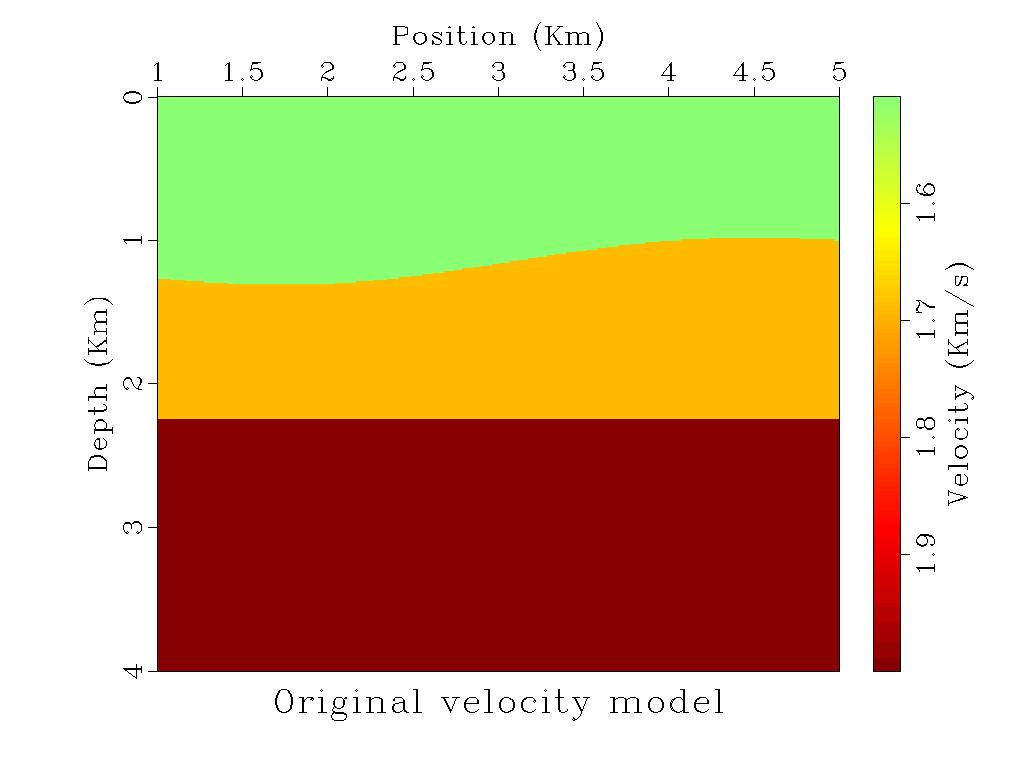
\includegraphics[scale=0.3]{images/mod1.jpeg}
\vspace{-0.3cm}
\end{center}
\begin{center}
 Fonte: Do Autor.
\end{center}
\label{fig:9.1}
\end{figure}

\begin{figure}[H]
\caption{Modelo de velocidades de três camadas com velocidades iguais a $1.508Km/s$,
$1.690Km/s$ e $2.000Km/s$, respectivamente. Este modelo é utilizado para a obtenção da seção
empilhada ERC através do empilhamento ERC.}
\begin{center}
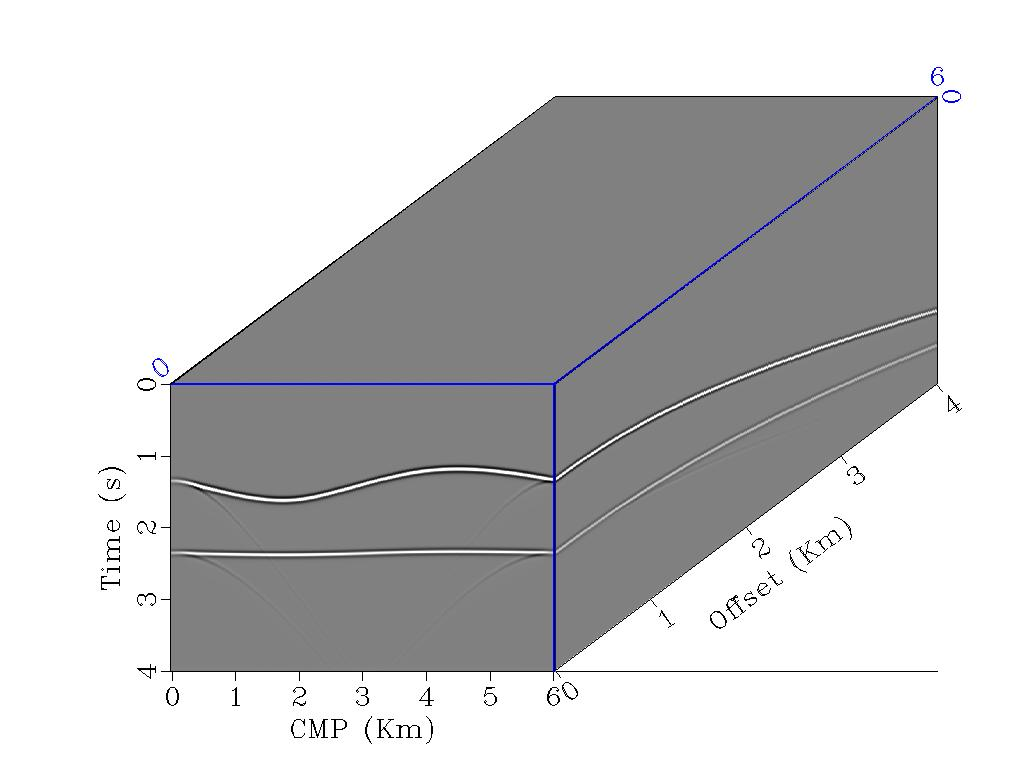
\includegraphics[scale=0.3]{images/datacube.jpeg}
\vspace{-0.3cm}
\end{center}
\begin{center}
 Fonte: Do Autor.
\end{center}
\label{fig:9.2}
\end{figure}

O nosso algoritmo para a inversão do modelo de velocidades em profundidade inicia com a obtenção dos dados
pré empilhados no domínio do PMC $m$ e do meio afastamento $h$ na Figura \ref{fig:9.2}. Estes dados foram
produzidos partir da modelagem Kirchhoff do modelo de velocidades
da Figura \ref{fig:9.1}. Este modelo possui três camadas com velocidades iguais a $1.508Km/s$,
$1.690Km/s$ e $2.000Km/s$, respectivamente. A modelagem Kirchhoff é feita através dos programas
de modelagem disponíveis no pacote de processamento sísmico Madagascar \cite{madagascar},
os mesmos utilizados no experimento numérico do Capítulo 6 para o refletor Gaussiano.

Em seguida, a partir dos dados sísmicos modelados, realizamos a otimização dos parâmetros $R_{NIP}$
e $\beta_0$ através do Very Fast Simulated Annealing (VFSA) e da utilização da aproximação de tempo
de trânsito do SRC não hiperbólico, com a metodologia descrita no Capítulo 4.
Estes parâmetros permitem a obtenção
das curvas de tempo de trânsito ERC para a realização do empilhamento das amplitudes. 
A próxima etapa consiste em estabelecer as famílias ERC onde são definidas as
curvas de tempo de trânsito ERC .

Assim, utilizamos a metodologia de interpolação com filtros FPE, descrita no Capítulo 4 e utilizada
no experimento numérico do Capítulo 7, para aumentar o número de amostras
dos dados modelados
no domínio do PMC, de modo a possibilitar amostragem suficiente para a
obtenção das famílias ERC e a subsequente obtenção da
seção de afastamento nulo através do empilhamento ERC. O empilhamento ERC
é realizado através da medida da coerência (semblance) das amplitudes sobre as curvas de tempo de trânsito
ERC em uma família ERC de traços sísmicos. As amplitudes são empilhadas sobre esta curva e atribuídas
às coordenadas ($m_0$,$t_0$) na seção empilhada ERC.
O algoritmo para a obtenção da seção empilhada ERC é apresentado no fluxograma a seguir.

\begin{figure}[H]
\caption{Representação esquemática do algoritmo para a obtenção da seção empilhada ERC
através do empilhamento ERC. Dados de entrada e saída de cada etapa do algoritmo.}
\begin{center}
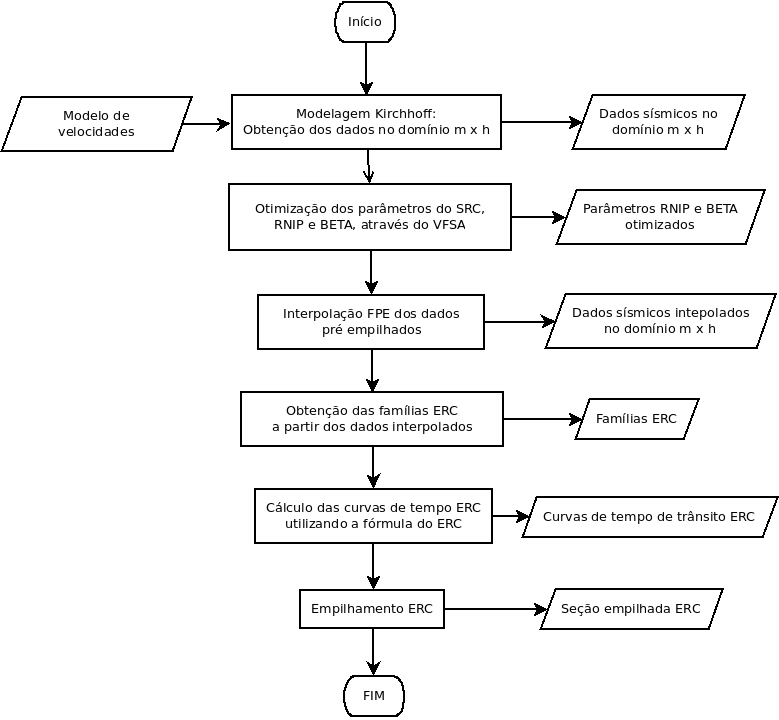
\includegraphics[scale=0.5]{images/fluxoemperc.png}
\vspace{-0.3cm}
\end{center}
\begin{center}
 Fonte: Do Autor.
\end{center}
\label{alg:9.1}
\end{figure}

\begin{figure}[H]
\caption{Seção empilhada ERC obtida através do empilhamento ERC
do modelo de velocidades da Figura \ref{fig:9.1}.}
\begin{center}
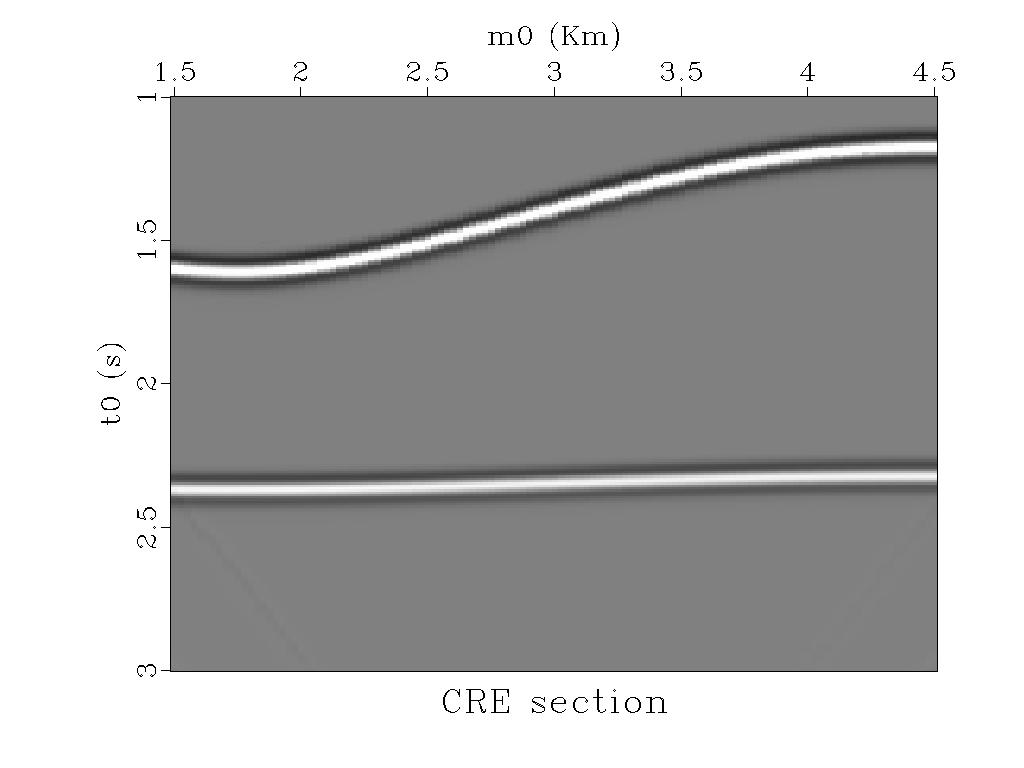
\includegraphics[scale=0.3]{images/stacked.jpeg}
\vspace{-0.3cm}
\end{center}
\begin{center}
 Fonte: Do Autor.
\end{center}
\label{fig:9.3}
\end{figure}

Após a obtenção da seção empilhada ERC através do empilhamento ERC dos dados sísmicos de reflexão
obtidos da modelagem Kirchhoff do modelo de velocidades da Figura \ref{fig:9.1},
com três camadas com as velocidades $1.508Km/s$, $1.690Km/s$ e $2.000Km/s$ respectivamente,
utilizando a metodologia de empilhamento ERC descrita no Capítulo 8,
realizamos o picking interativo dos tempos de trânsito, selecionando manualmente alguns
pontos sobre os refletores na seção empilhada ERC
(Ver Figura \ref{fig:9.4}, pontos em amarelo).
Estes tempos de trânsito selecionados na seção de afastamento nulo (seção empilhada ERC)
são os tempos duplos $t_0$ dos raios normais que partem da coordenada $m_0$
de um PMC na superfície de aquisição e incidem normais ao refletor no ponto PIN (Figura \ref{fig:9.5}).

Os tempos de trânsito $t_0$ escolhidos são utilizados para traçar raios normais
a partir da superfície de aquisição em direção ao modelo de velocidades
em profundidade,
de modo a determinar a possível localização do refletor no modelo
para um determinado modelo de velocidades.
O traçamento continua até que metade do tempo de trânsito $t_0$ seja consumido.
O modelo de velocidades inicial é um modelo de velocidade constante igual à velocidade $v_0$
próxima da superfície de aquisição.

\begin{figure}[H]
\caption{Picking manual dos tempos de trânsito sobre um refletor da seção empilhada ERC. Os pontos
em amarelo são os pares $t_0$ e $m_0$ escolhidos.}
\begin{center}
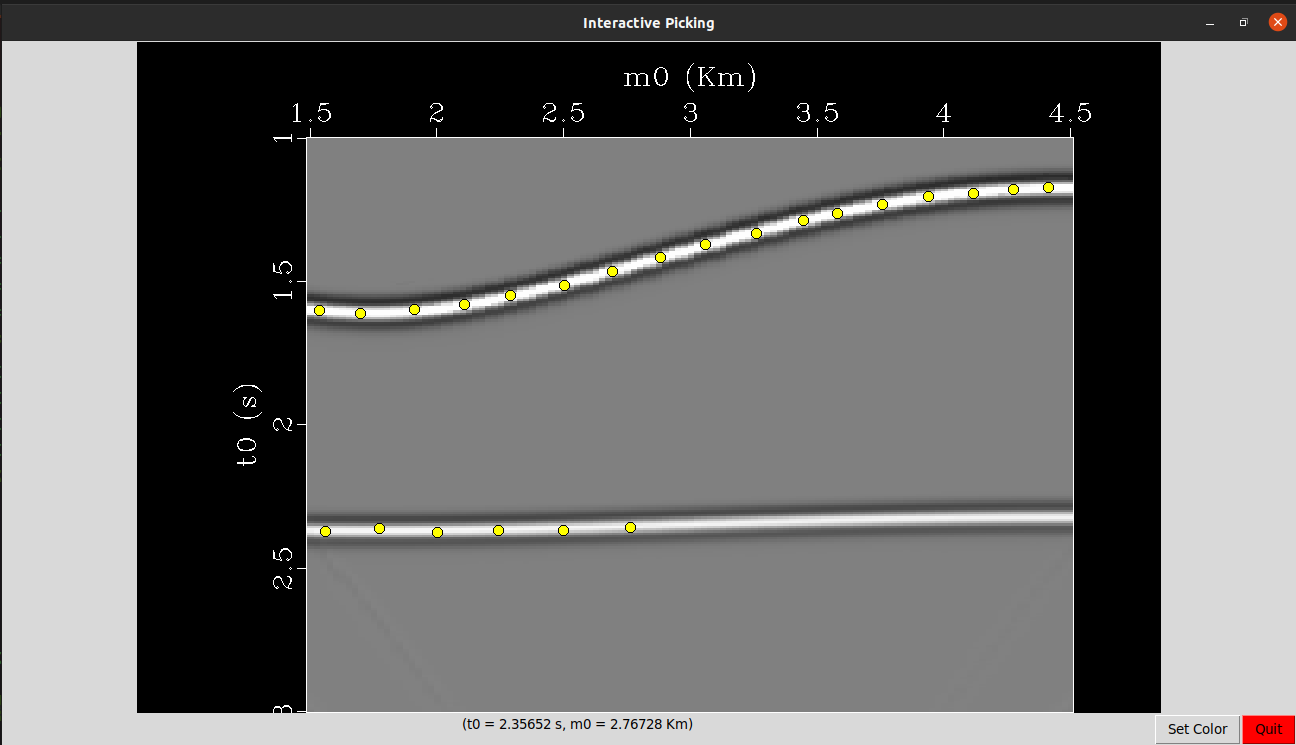
\includegraphics[scale=0.3]{images/picking.png}
\vspace{-0.3cm}
\end{center}
\begin{center}
 Fonte: Do Autor.
\end{center}
\label{fig:9.4}
\end{figure}

\begin{figure}[H]
\caption{Exemplo esquemático do traçamento de raios normais a partir de uma coordenada de um CMP $m_0$
na superfície de aquisição em direção ao modelo em profundidade.
O raio normal (seta) parte da superfície de aquisição com ângulo $\beta_0$ e incide normal
ao refletor no Ponto de Incidência Normal (PIN).}
\begin{center}
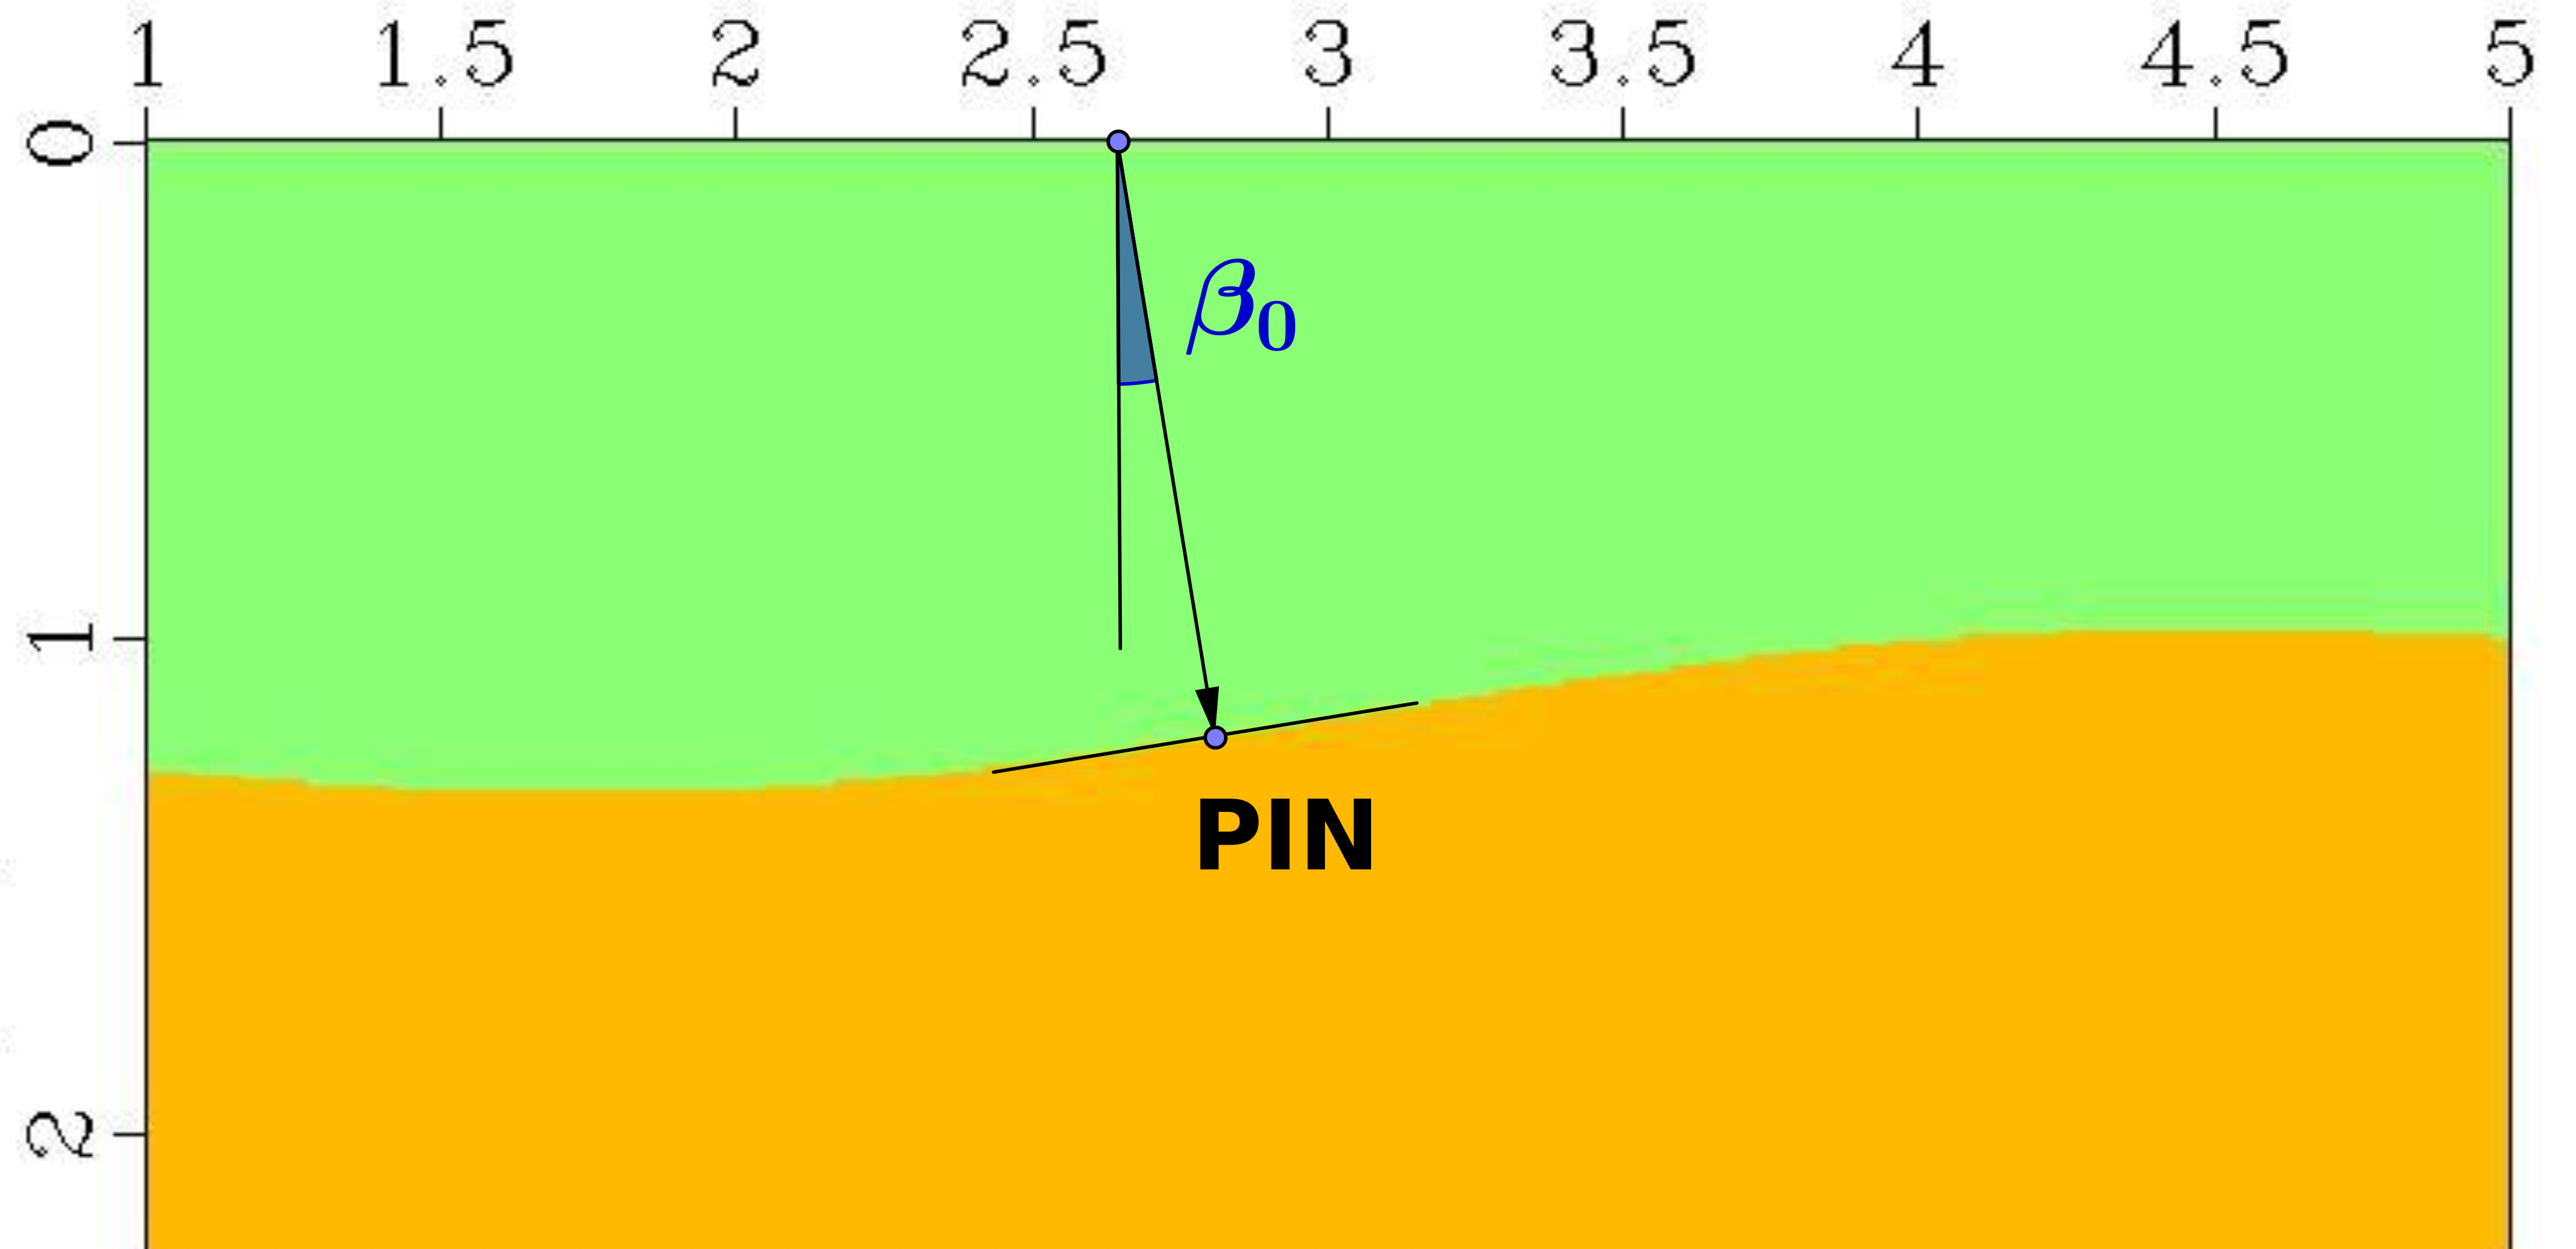
\includegraphics[scale=0.5]{images/modelagem.png}
\vspace{-0.3cm}
\end{center}
\begin{center}
 Fonte: Do Autor.
\end{center}
\label{fig:9.5}
\end{figure}

\begin{figure}[H]
\caption{Exemplo de traçamento do raio utilizando o programa \textit{sfrays2}
em direção a um modelo de velocidades suavizado.
Este programa está disponível no pacote de processamento sísmico Madagascar e foi
modificado para obter a localização das fontes PIN nos modelos de velocidade deste relatório.}
\begin{center}
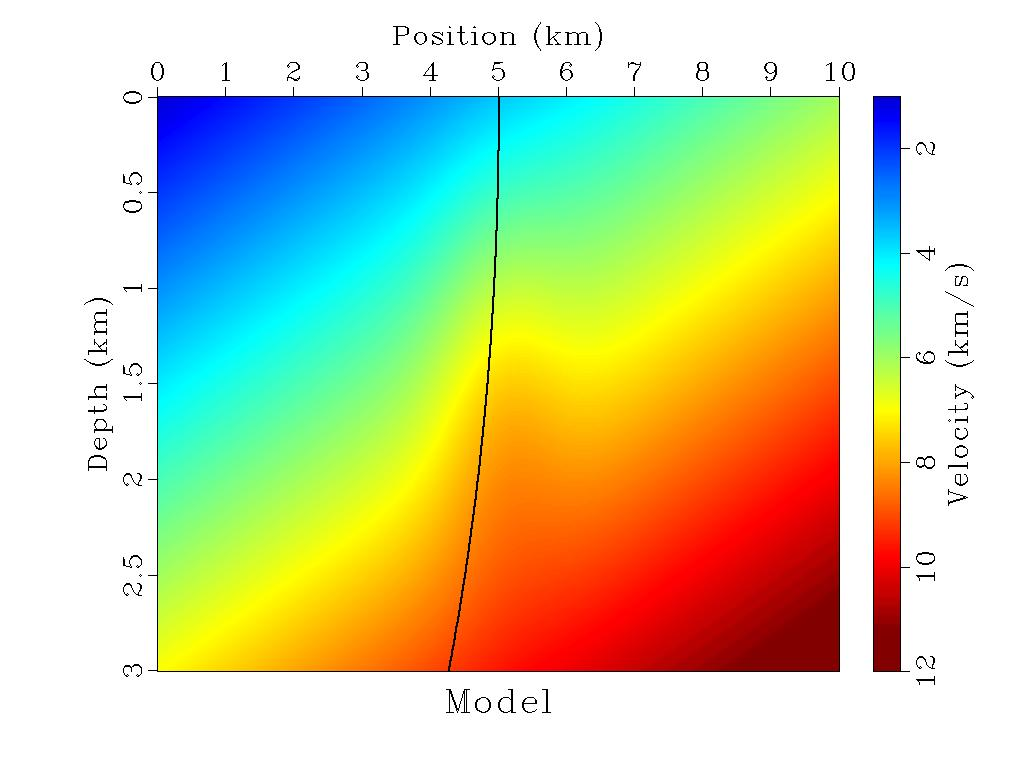
\includegraphics[scale=0.3]{images/raiomodelo.jpg}
\vspace{-0.3cm}
\end{center}
\begin{center}
 Fonte: Do Autor.
\end{center}
\label{fig:9.6}
\end{figure}

\begin{figure}[H]
\caption{Exemplo de traçamento do raio utilizando o programa \textit{sfrays2}
de um ponto no modelo de velocidades suavizado em direção à superfície de aquisição.
Este programa está disponível no pacote de processamento sísmico Madagascar e foi
modificado para a realização da modelagem direta neste relatório.}
\begin{center}
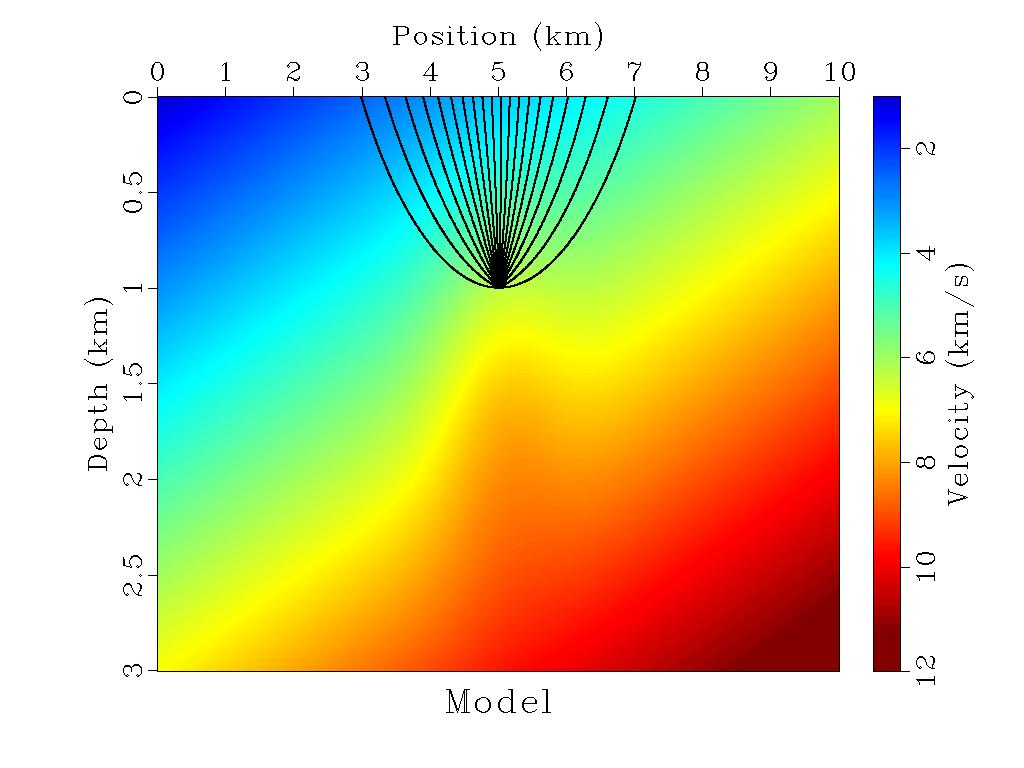
\includegraphics[scale=0.3]{images/raioleque.jpg}
\vspace{-0.3cm}
\end{center}
\begin{center}
 Fonte: Do Autor.
\end{center}
\label{fig:9.7}
\end{figure}

O programa para o traçamento de raios foi desenvolvido
utilizando as interfaces da Application Programming Interface (API)
do pacote de processamento sísmico Madagascar\footnote{Este pacote de processamento sísmico
está disponíveil no site oficial do pacote Madagascar em \url{http://www.ahay.org/wiki/Main_Page}. 
Os programas do pacote e a interface de traçamento de raios é disponibilizada sob
os termos da licensa de uso GPL-3.0 para software livre disponível
em \url{https://www.gnu.org/licenses/gpl-3.0.txt}.} \cite{madagascar}
e da construção de uma versão modificada do programa para traçamento de raios 
\textit{sfrays2} que realiza o traçamento cinemático dos raios
através do método Runge-Kutta. Estes raios podem ser traçados da superfície de aquisição em
direção ao modelo de velocidades em profundidade (Figura \ref{fig:9.6}) e de um
ponto no modelo de velocidades em direção à superfície de aquisição (Figura \ref{fig:9.7}).
O programa também permite obter as coordenadas de chegada dos raios e o tempo de trânsito.

Cada raio normal é iniciado na superfície de aquisição na posição da coordenada $m_0$ e lançado no modelo 
com a direção inicial dada pelo parâmetro $\beta_0$ (Figura \ref{fig:9.5}).
O ponto final do raio é a possível localização do refletor em profundidade
e onde será estabelecida a localização das fontes pontuais PIN para o modelo de velocidades.
O vetor vagarosidade neste ponto é
normal ao refletor, e com estas informações, o modelo de velocidades inicial é configurado \cite{niptomo}.

\begin{figure}[H]
\caption{Exemplo esquemático do traçamento de raios a partir do ponto PIN em profundidade.
Os raios são lançados com o mesmo ângulo $\theta_i$ em relação à normal ao refletor no ponto
PIN de modo a simular raios de reflexão de uma família ERC que atingem a superfície de aquisição
na posição da fonte $x_s$ e do receptor $x_r$.}
\begin{center}
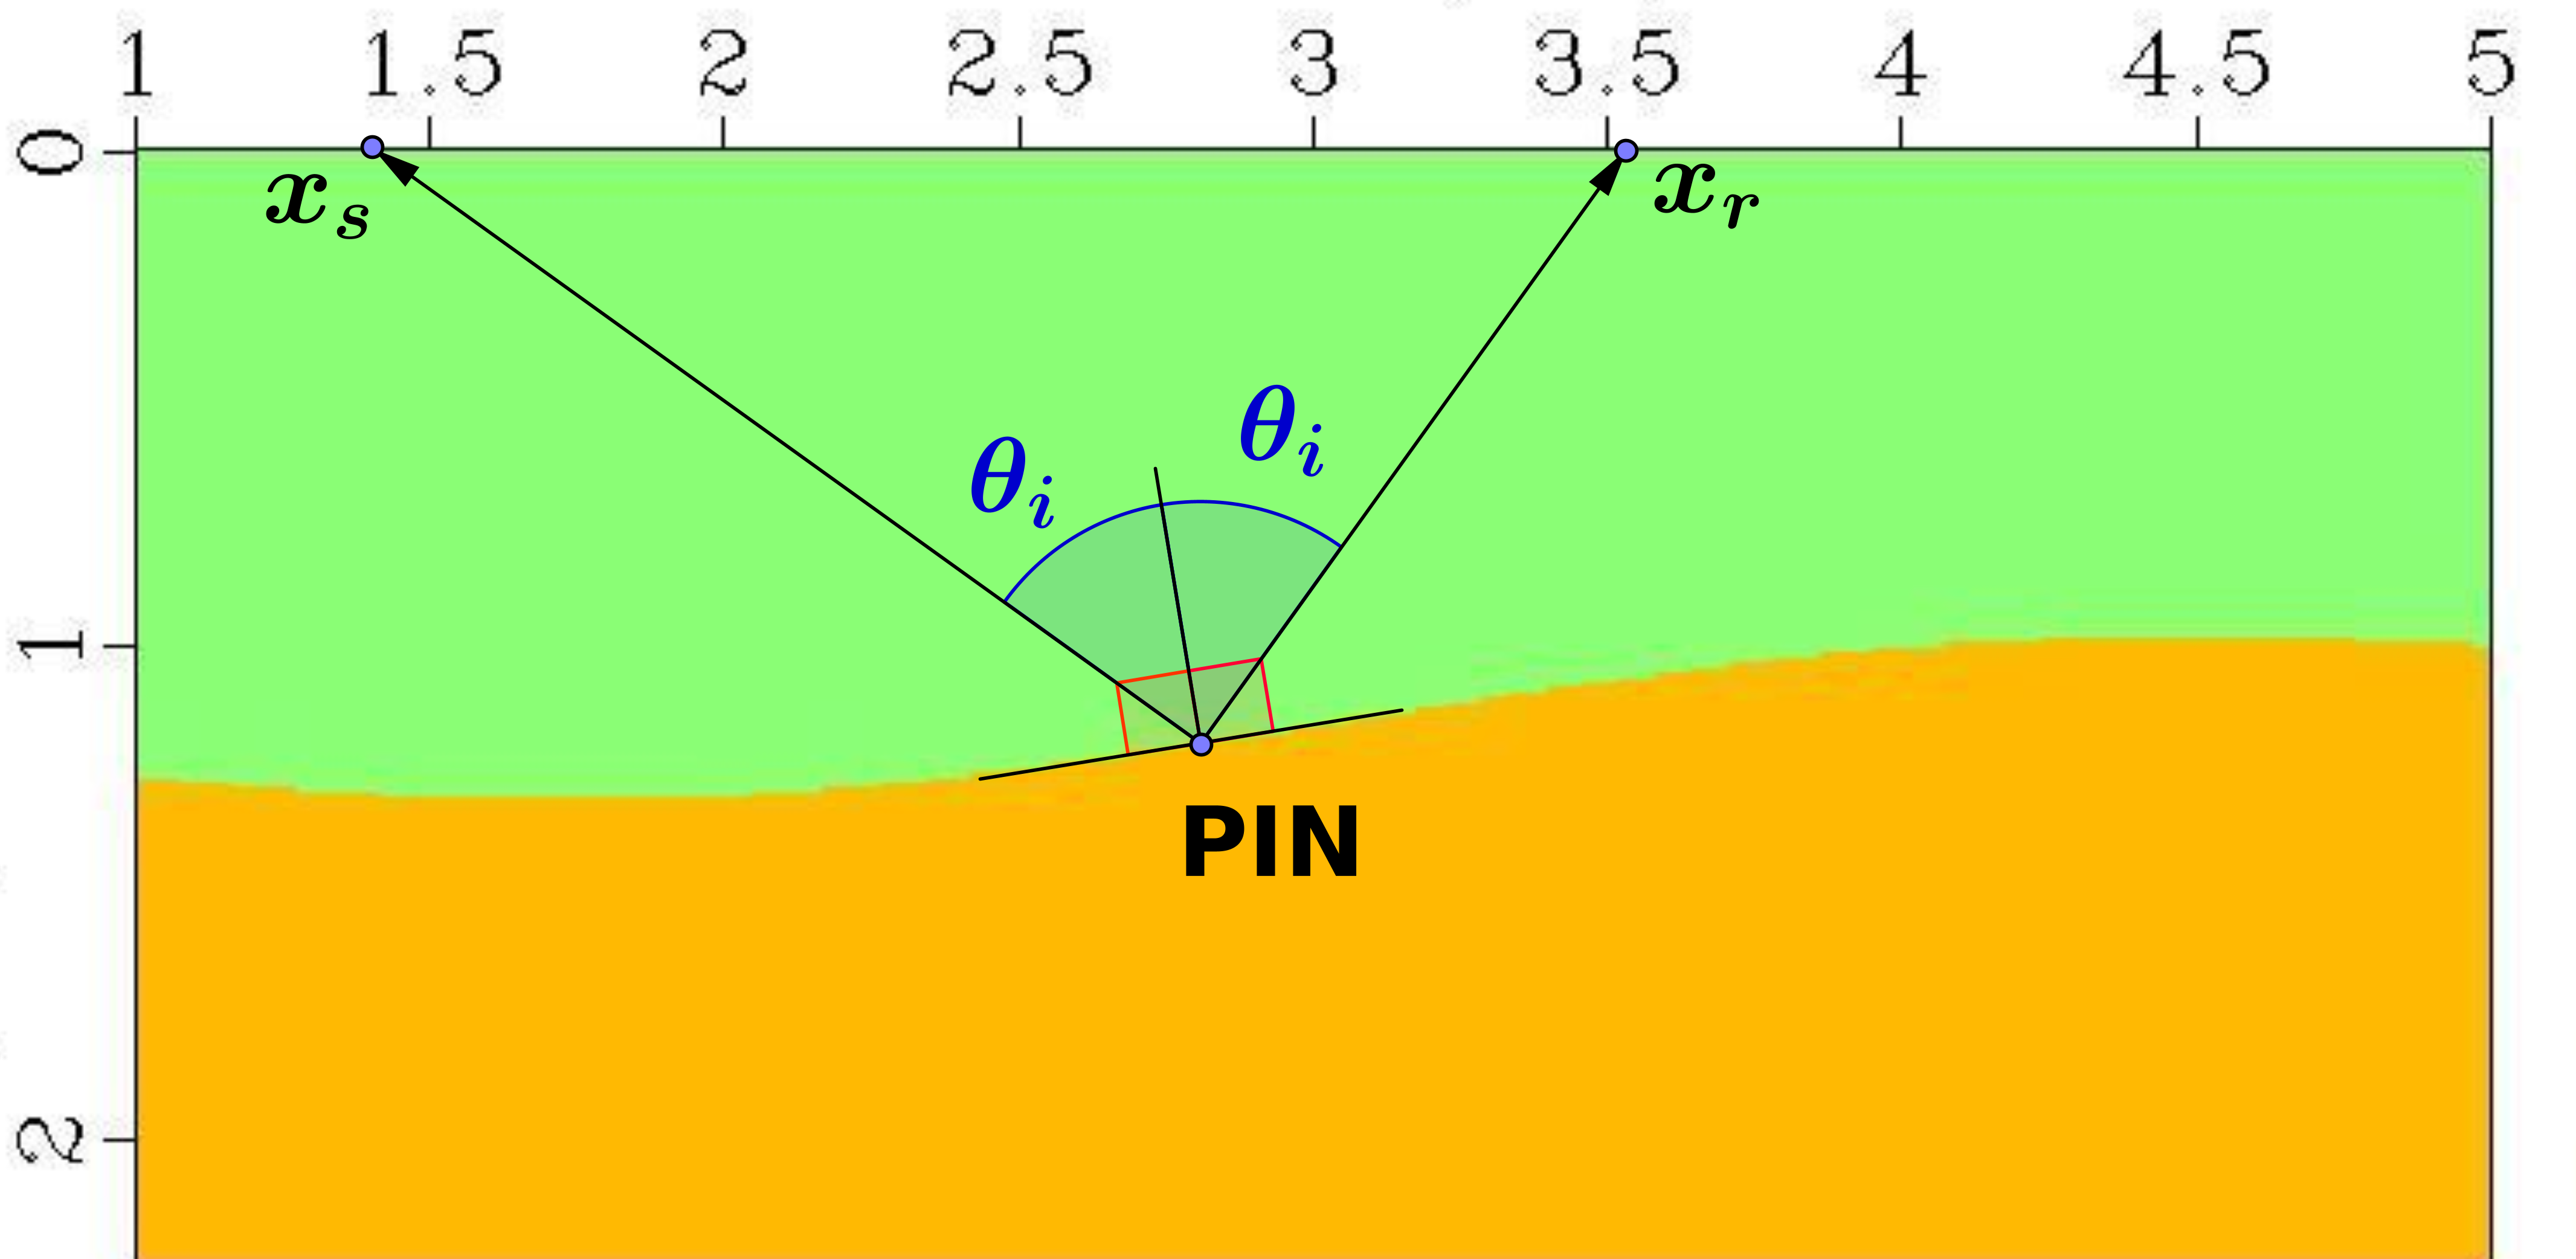
\includegraphics[scale=0.5]{images/modelagem2.png}
\vspace{-0.3cm}
\end{center}
\begin{center}
 Fonte: Do Autor.
\end{center}
\label{fig:9.8}
\end{figure}

Após a determinação da localização das fontes no modelo,
a modelagem direta é realizada através do traçamento de pares de raios de reflexão
iniciando nas posições das fontes PIN determinadas para um modelo de velocidades
inicial,
simulando uma família ERC de raios de reflexão que atingem a superfície de aquisição
na posição da fonte $x_s$ e do receptor $x_r$ (Figura \ref{fig:9.8}).
Este leque de raios é lançado em direção à superfície de aquisição,
os tempos de trânsito dos raios de reflexão são armazenados \cite{stereo}.
Os tempos de trânsito dos raios de reflexão obtidos no traçamento de raios são comparados com os tempos
de trânsito da aproximação de tempo de trânsito ERC a seguir \cite{cre}:

\begin{multline}
\label{eq:9.1}
t(h,m)= \left( \tau_0-\frac{2R_{NIP}}{v_0} \right) 
+\frac{R_{NIP}}{v_0}\sqrt{1-2\alpha(m-m_0+h)+\frac{(m-m_0+h)^2}{R_{NIP}^2}} \\
+\frac{R_{NIP}}{v_0}\sqrt{1+2\alpha(m-m_0-h)+\frac{(m-m_0-h)^2}{R_{NIP}^2}}
\end{multline}


Onde $m$ é a coordenada do PMC, $h$ é a coordenada do afastamento entre fonte e receptor e
$\alpha$ é um parâmetro de assimetria dado em função de $R_{NIP}$ e $\beta_0$.
As diferenças $e_i$ entre os tempos de trânsito do traçamento de raios e dos tempos de trânsito
calculados são somadas segundo a fórmula \cite{stoffa}:

\begin{equation}
\label{eq:9.2}
L_2 = \left[ \sum_{i=1}^{ND} |e_i|^2 \right]^\frac{1}{2}
\end{equation}

As posições $x_s$ e $x_r$ são dadas pelo traçamento de raios armazenando as coordenadas de chegada
na superfície de aquisição dos raios de reflexão simulados na modelagem direta. Estas coordenadas podem
ser transformadas nas coordenadas do afastamento $h$ e PMC $m$ pelas Equações a seguir:

\begin{equation}
\label{eq:9.3}
h = (x_r-x_s)/2
\end{equation}

\begin{equation}
\label{eq:9.4}
m = (x_r+x_s)/2
\end{equation}

Como $\beta_0$, $R_{NIP}$ são parâmetros conhecidos para cada raio normal e obtidos do empilhamento
ERC e $v_0$ é a velocidade próximo da superfície de aquisição, também conhecida, podemos calcular o
tempo de trânsito esperado com a Equação \ref{eq:9.1} e comparar com o tempo de trânsito do raio de
reflexão simulado
dado pela soma dos tempos $\Delta \tau_s$ e $\Delta \tau_r$,
do raio que sai do ponto PIN e chega em $x_s$
e do raio
que sai do ponto PIN e chega em $x_r$, respectivamente.
Esta diferença deve ser mínima para o modelo de velocidades
correto. A soma dos tempos de trânsito obtidas com o
traçamento de raios é dada a seguir:

\begin{equation}
\label{eq:9.5}
\tau(h,m) = \Delta \tau_s + \Delta \tau_r
\end{equation}

Assim, a diferença $e_i$ e a norma dois $L_2$ da Equação \ref{eq:9.2} podem ser estabelecidas como:

\begin{equation}
\label{eq:9.6}
L_2 = \left[ \sum_{i=1}^{ND} |e_i|^2 \right]^\frac{1}{2}
= \left[ \sum_{i=1}^{ND} |\tau(h,m)-t(h,m)|^2 \right]^\frac{1}{2}
\end{equation}

A norma dois das diferenças nos tempos de trânsito (Equação \ref{eq:9.2})
será utilizada como critério de
convergência do modelo de velocidades: O modelo de velocidades otimizado deverá produzir
o valor mínimo das diferenças entre os tempos de trânsito obtidos com o traçamento de raios
e calculados com a fórmula do ERC (Equação \ref{eq:9.1}). Assim, a estratégia de inversão consiste em
atualizar o modelo de velocidades utilizado de modo a
encontrar o modelo que produz o mínimo global da Equação \ref{eq:9.2}. O algoritmo de inversão
do modelo de velocidades é apresentado na Figura \ref{fig:9.9}.

A metodologia para a atualização do modelo de velocidades durante a inversão é utilizar o
Very Fast Simulated Annealing (VFSA) para atualizar parâmetros que definem o modelo de velocidades
em profundidade tomando como critério de convergência o valor calculado para a norma dois na Equação
\ref{eq:9.2}. Os parâmetros irão depender do modo de representação do modelo de velocidades, exemplo:
um modelo de velocidades em que a velocidade cresce linearmente com a profundidade depende do gradiente
de velocidades $g_z$ e da velocidade próximo da superfície de aquisição $v_0$. Considerando $v_0$ conhecida,
a atualização do modelo será dada pela atualização do gradiente $g_z$ como parâmetro otimizado pelo VFSA.

Esta estratégia de otimização é realizada em looping (Figura \ref{fig:9.10}),
utilizando o modelo de velocidades otimizado, resultado
da otimização anterior, como novo modelo de velocidades inicial. Assim, a localização das fontes PIN é
atualizada no início do processo de inversão para cada novo modelo de velocidades inicial utilizado.
Também ocorre a atualização do vetor vagarosidade na localização da fonte PIN e consequentemente
dos ângulos de chegada do raio normal nestes pontos.

\begin{figure}[H]
\caption{Representação esquemática do algoritmo de inversão do modelo de velocidades
a partir da estratégia apresentada neste capítulo.}
\begin{center}
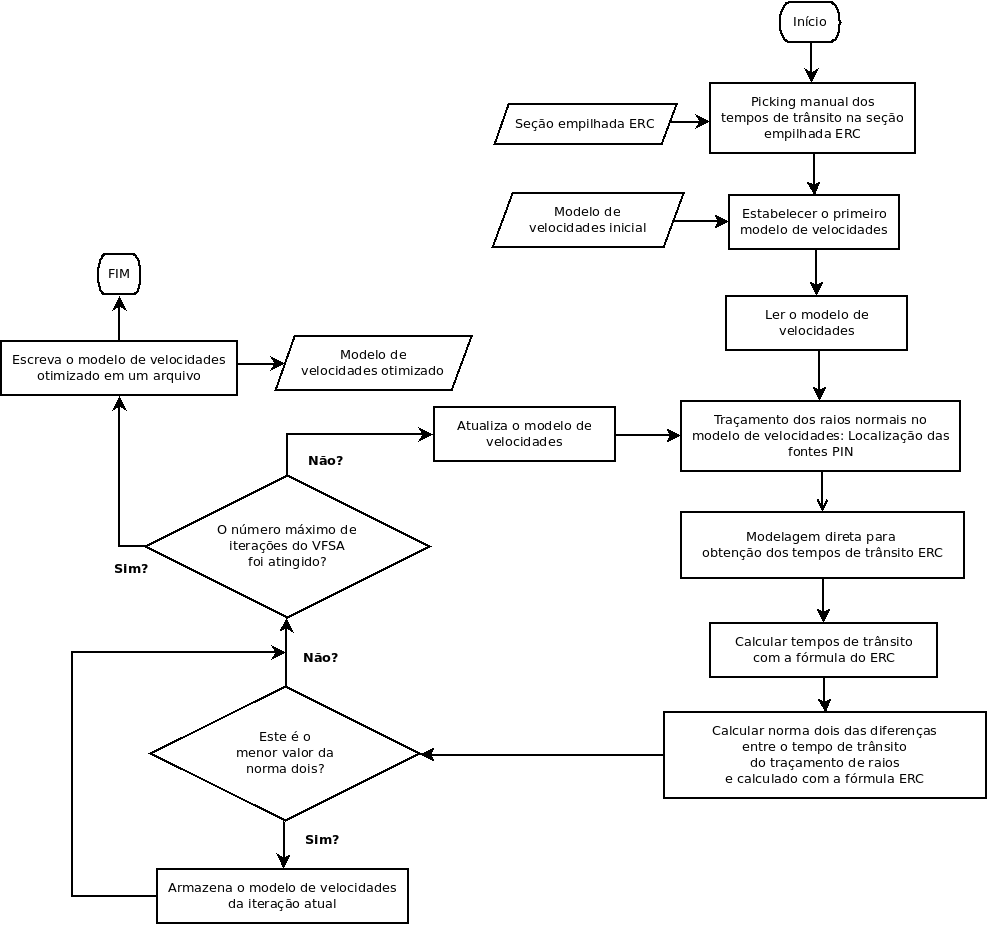
\includegraphics[scale=0.45]{images/fluxocomp.png}
\vspace{-0.3cm}
\end{center}
\begin{center}
 Fonte: Do Autor.
\end{center}
\label{fig:9.9}
\end{figure}

\begin{figure}[H]
\caption{Representação esquemática do algoritmo de inversão do modelo de velocidades
sendo utilizado em looping. O modelo de velocidades otimizado da iteração anterior é utilizado
como novo modelo de velocidades inicial e inversão é refeita.}
\begin{center}
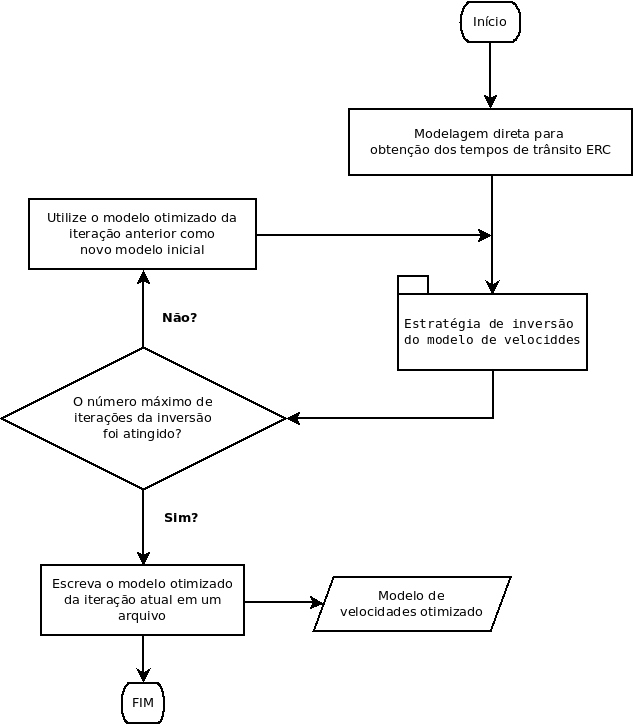
\includegraphics[scale=0.5]{images/fluxorepeat.png}
\vspace{-0.3cm}
\end{center}
\begin{center}
 Fonte: Do Autor.
\end{center}
\label{fig:9.10}
\end{figure}
 % Proposta de uma metodologia para inversão do modelo de velocidades
\chapter{MODELO DE VELOCIDADES DE BACKGROUND}
\label{cap10}

A primeira iteração do algoritmo de inversão tem por objetivo a obtenção do gradiente de
velocidades em profundidade do modelo de velocidades de background \cite{niptomo,stereo}.
O modelo inicial utilizado é um modelo de velocidades homogêneo
e de velocidade constante igual a $1.5Km/s$,
correspondente a velocidade próxima da superfície de aquisição. Traçamos raios normais
partindo da coordenada $m_0$ e com ângulo de inclinação $\beta_0$ em direção ao modelo
de velocidade constante para determinar a localização inicial das fontes PIN (cruzes
em preto na Figura \ref{fig:10.1}). Este será o modelo inicial desta etapa da inversão.

\begin{figure}[H]
\caption{Modelo de velocidade constante utilizado para a configuração inicial da
posição das fontes pontuais PIN (cruzes em preto).}
\begin{center}
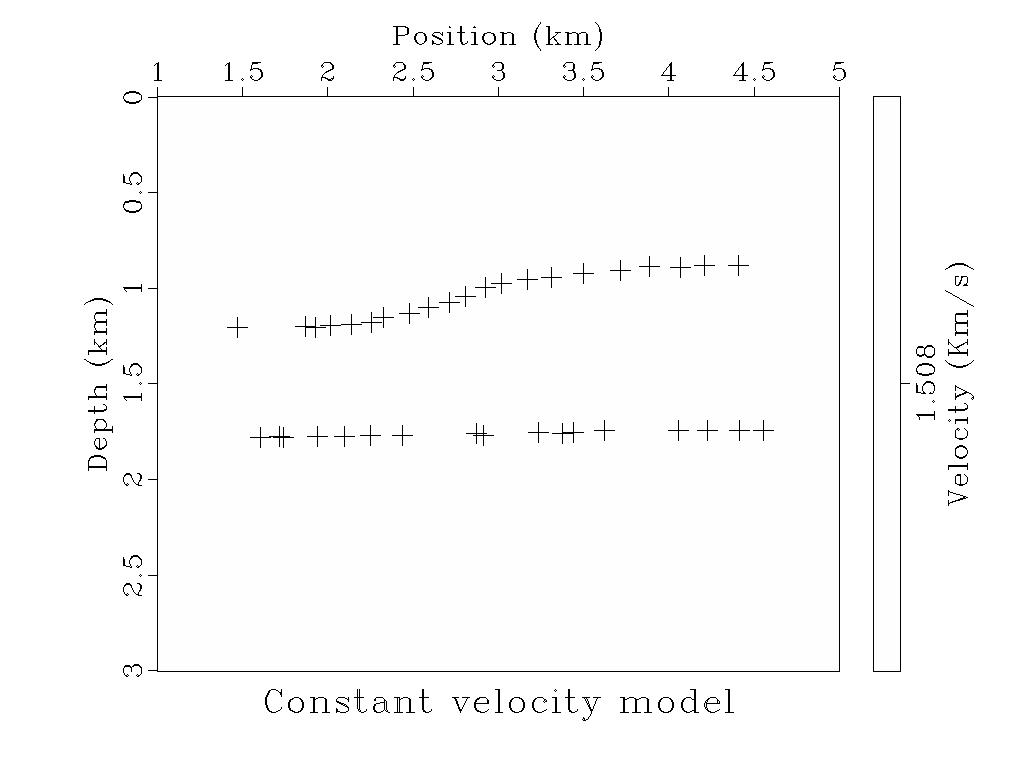
\includegraphics[scale=0.3]{images/ctevel.jpeg}
\vspace{-0.3cm}
\end{center}
\begin{center}
 Fonte: Do Autor.
\end{center}
\label{fig:10.1}
\end{figure}

Para a otimização do modelo de velocidades de gradiente constante
é utilizada a Equação \ref{eq:9.2} da soma das
diferenças nos tempos de trânsito obtidos com o traçamento de raios e os tempos de trânsito calculados utilizando a fórmula do ERC (Equação \ref{eq:9.1}). Utilizamos o algoritmo Very Fast Simulated Annealing (VFSA) para atualizar o gradiente em profundidade do modelo de velocidades (Ver o algoritmo completo na
Figura \ref{fig:10.2}).

\begin{figure}[H]
\caption{Representação esquemática do algoritmo de inversão do gradiente $g_z$ do modelo de velocidades
com gradiente constante (velocidade cresce linearmente com a profundidade).}
\begin{center}
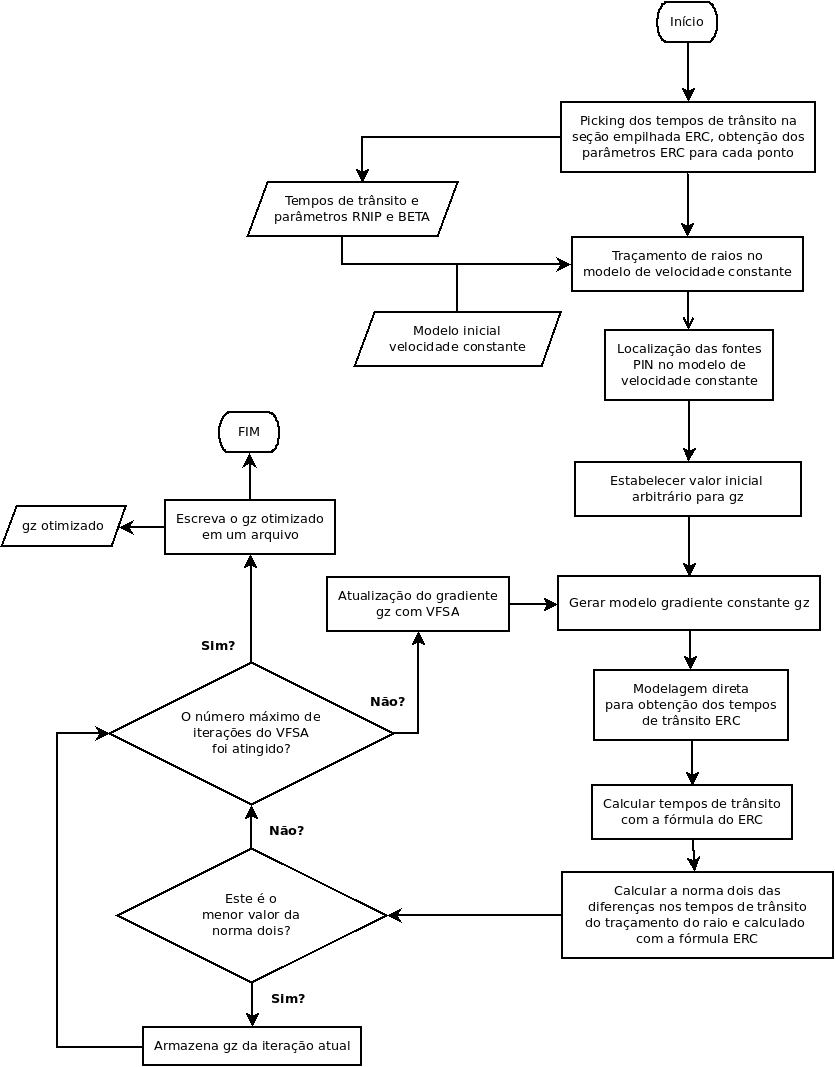
\includegraphics[scale=0.5]{images/fluxogz.png}
\vspace{-0.3cm}
\end{center}
\begin{center}
 Fonte: Do Autor.
\end{center}
\label{fig:10.2}
\end{figure}

O modelo de velocidades é atualizado a cada iteração do algoritmo para cada valor do gradiente $g_z$
dada a seguinte função de velocidades:

\begin{equation}
\label{eq:10.1}
v(z)=z g_z+v_0
\end{equation}

Em \ref{eq:10.1} a velocidade $v(z)$ cresce linearmente com a profundidade e $v_0$
é o valor da velocidade próximo da superfície.

O valor mínimo da diferença entre os tempos de trânsito (Equação \ref{eq:9.2})
será obtido para o gradiente de velocidades ótimo.
O valor do gradiente é armazenado e utilizado para gerar o modelo de velocidades
da Figura \ref{fig:10.3}. Este modelo será o modelo de background utilizado na etapa seguinte
da inversão do modelo de velocidades com variação lateral de velocidade.

O gradiente de velocidades obtido é $g_z=0.1673 s^{-1}$. O modelo de velocidades resultante é apresentado na
Figura \ref{fig:10.3} à direita em comparação com o modelo de velocidade constante na Figura \ref{fig:10.3}
à esquerda, as cruzes em preto representam a localização das fontes pontuais PIN em cada um dos modelos.
A localização das fontes pontuais PIN obtidas a partir do modelo de velocidades de gradiente constante
é plotada sobre o modelo de velocidades original na Figura \ref{fig:10.4}.

\begin{figure}[H]
\caption{Modelo de velocidade constante à esquerda (velocidade igual a $1.5Km/s$)
e o modelo de velocidades com gradiente constante à direita
(o gradiente de velocidades em profundidade é $0.1673 s^{-1}$).
As cruzes em preto representam a localização das fontes PIN.}
\begin{center}
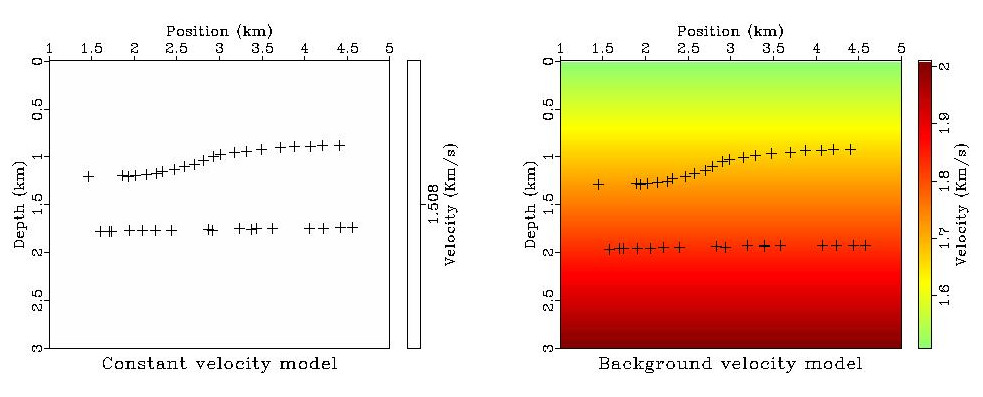
\includegraphics[scale=2]{images/compare.jpeg}
\vspace{-0.3cm}
\end{center}
\begin{center}
 Fonte: Do Autor.
\end{center}
\label{fig:10.3}
\end{figure}

\begin{figure}[H]
\caption{Localização das fontes pontuais PIN (cruzes em preto)
obtidas com o modelo de velocidades de gradiente
constante plotadas sobre o modelo de velocidades original.
Compare a localização das cruzes com a posição dos refletores.}
\begin{center}
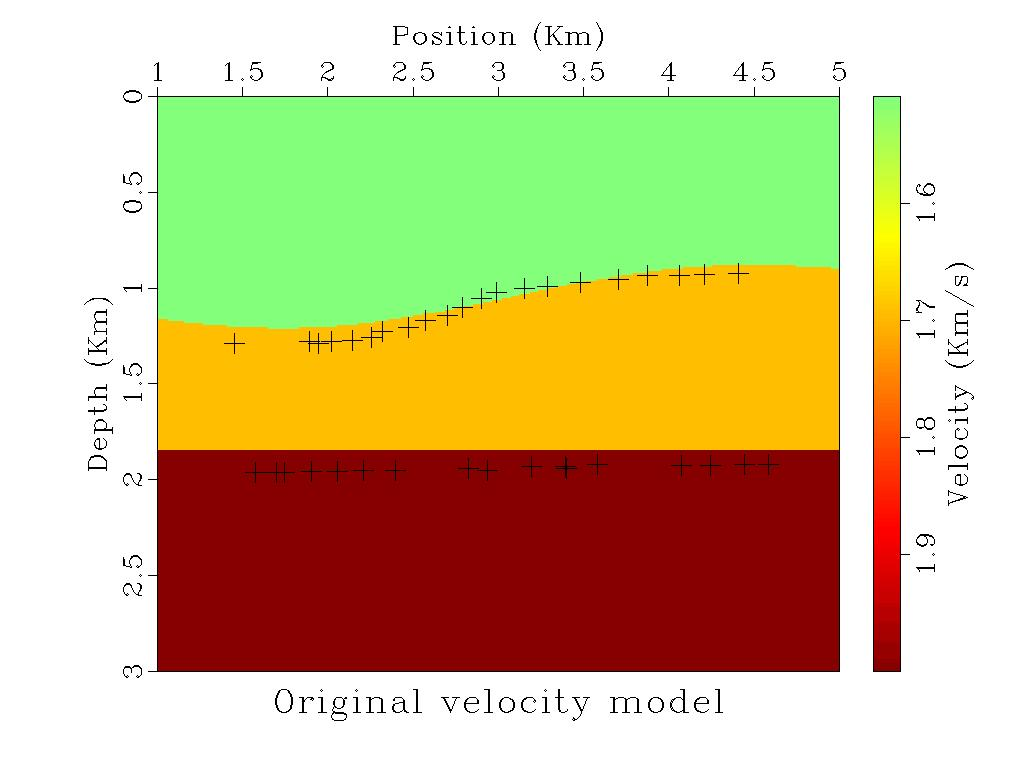
\includegraphics[scale=0.3]{images/gzvel.jpeg}
\vspace{-0.3cm}
\end{center}
\begin{center}
 Fonte: Do Autor.
\end{center}
\label{fig:10.4}
\end{figure}


\begin{figure}[H]
\caption{Localização das fontes PIN obtidas no modelo de velocidade constante
plotadas sobre o modelo de velocidades original (à esquerda)
e localização das fontes PIN obtidas no modelo de velocidades com gradiente constante
plotadas sobre o modelo de velocidades original (à direita).
As cruzes em preto representam a localização das fontes PIN.}
\begin{center}
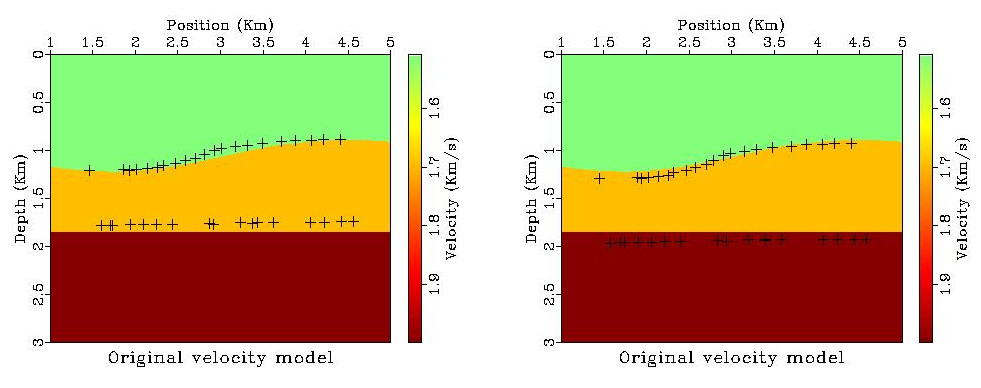
\includegraphics[scale=2]{images/resultinv.jpeg}
\vspace{-0.3cm}
\end{center}
\begin{center}
 Fonte: Do Autor.
\end{center}
\label{fig:10.5}
\end{figure}

\chapter{MODELO DE VELOCIDADES COM VARIAÇÃO LATERAL}
\label{cap11}

Esta etapa do desenvolvimento da tese ainda não está totalmente concluída. Neste capítulo apresentamos
os resultados preliminares:
A segunda etapa da estratégia de inversão do modelo de velocidades consiste em encontrar a perturbação
$\delta v(x,z)$ para um modelo de velocidades de background arbitrário.
Utilizamos o modelo de velocidades de gradiente constante (Figura \ref{fig:10.2} à direita)
obtido na etapa de inversão do Capítulo 10. O objetivo desta etapa é obter a correta 
localização das fontes PIN sobre os refletores do modelo de velocidades original (Figura \ref{fig:9.2}).
Assim, definimos o novo modelo de velocidades com variação lateral de velocidade na
Equação a seguir:

\begin{equation}
\label{eq:11.1}
v(x,z)=z g_z+v_0+\delta v(x,z)
\end{equation}

Onde $z$ é a coordenada da profundidade, $g_z$ é o gradiente de velocidades em profundidade obtido na
etapa de inversão anterior e $v_0$ é a velocidade próxima da superfície. O termo $\delta v(x,z)$ representa
a perturbação no modelo de velocidades de background (Equação \ref{eq:10.1})
representado pelas duas primeiras parcelas à direita na 
Equação \ref{eq:11.1}.

A otimização do modelo de velocidades
representado pela Equação \ref{eq:11.1}
é realizada de forma semelhante à desenvolvida no Capítulo 10:
Utilizamos a Equação \ref{eq:9.2} da soma das diferenças nos tempos de trânsito obtidos com o traçamento de raios no modelo de velocidades e os tempos de trânsito calculados utilizando a fórmula do ERC
(Equação \ref{eq:9.1}) como critério de convergência.
Todavia, nesta etapa, o algoritmo Very Fast Simulated Annealing (VFSA) é utilizado para realizar a otimização das perturbações $\delta v(x,z)$ do modelo de velocidades ao invés do gradiente de velocidades em
profundidade, já obtido na etapa anterior. Estas perturbações são atualizadas a cada iteração do VFSA (Ver a estratégia completa na representação esquemática do algoritmo na Figura \ref{fig:11.1}).

Ainda precisamos escolher a melhor estratégia para a representação do modelo de velocidades
e para a interpolação dos pontos sobre a malha. Temporariamente, utilizamos a representação
das perturbações do modelo de velocidades de background em uma malha regular de pontos de
controle $\Delta v_{ij}$. Somamos estas perturbações ao modelo de background nos pontos sobre
a malha utilizando a Equação \ref{eq:11.1} e interpolamos para todo o modelo de velocidades
através da interpolação essentially non-oscillatory (ENO) \cite{eno1,eno2}. Esta metodologia
de interpolação é utilizada para restringir o número de parâmetros a serem otimizados pelo VFSA
aos pontos de controle ao invés de otimizar todos os pontos sobre a malha do modelo de velocidades,
pois um número grande de parâmetros pode prejudicar a otimização com o VFSA.

\begin{figure}[H]
\caption{Representação esquemática do algoritmo de inversão do modelo de velocidades
com variação lateral de velocidade.}
\begin{center}
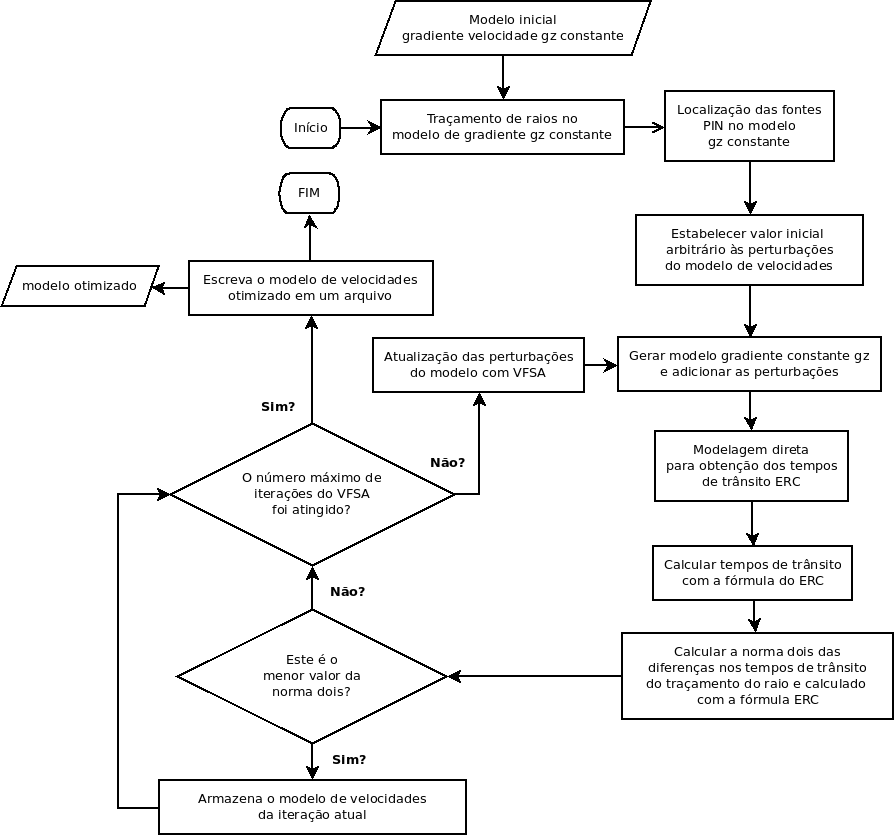
\includegraphics[scale=0.5]{images/fluxoinv.png}
\vspace{-0.3cm}
\end{center}
\begin{center}
 Fonte: Do Autor.
\end{center}
\label{fig:11.1}
\end{figure}

Assim, a Equação \ref{eq:11.1} se torna, para os nós da malha de pontos de controle:

\begin{equation}
\label{eq:11.2}
v_{ij}(x_j,z_i)=z_i g_z+v_0+\delta v_{ij}
\end{equation}

Deste modo, a estratégia de inversão do modelo de velocidades consiste em obter
as perturbações $\delta v_{ij}$ do modelo de velocidades de background (Equação \ref{eq:11.2})
de modo a produzir a melhor localização das fontes PIN sobre os refletores em profundidade.
A velocidade próxima à superfície $v_0$ e o gradiente de velocidades $g_z$ são constantes conhecidas
e definem o modelo de velocidades de background.

\begin{figure}[H]
\caption{Resultado da inversão do modelo de velocidades. Houve considerável melhora na
localização das fontes PIN (cruzes em preto) sobre os refletores em profundidade.}
\begin{center}
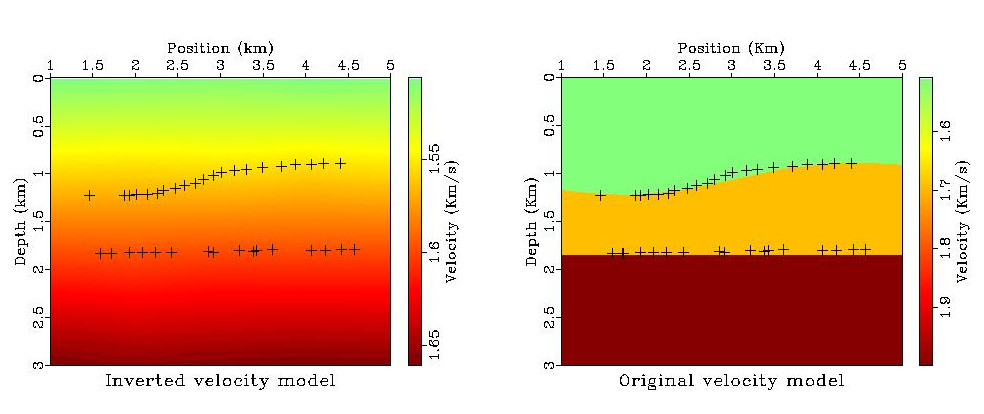
\includegraphics[scale=2]{images/inverted-original.jpeg}
\vspace{-0.3cm}
\end{center}
\begin{center}
 Fonte: Do Autor.
\end{center}
\label{fig:11.2}
\end{figure}

\begin{figure}[H]
\caption{Resultado da localização das fontes PIN (cruzes em preto)
para o modelo de velocidades de gradiente constante sobre o modelo de velocidades original.}
\begin{center}
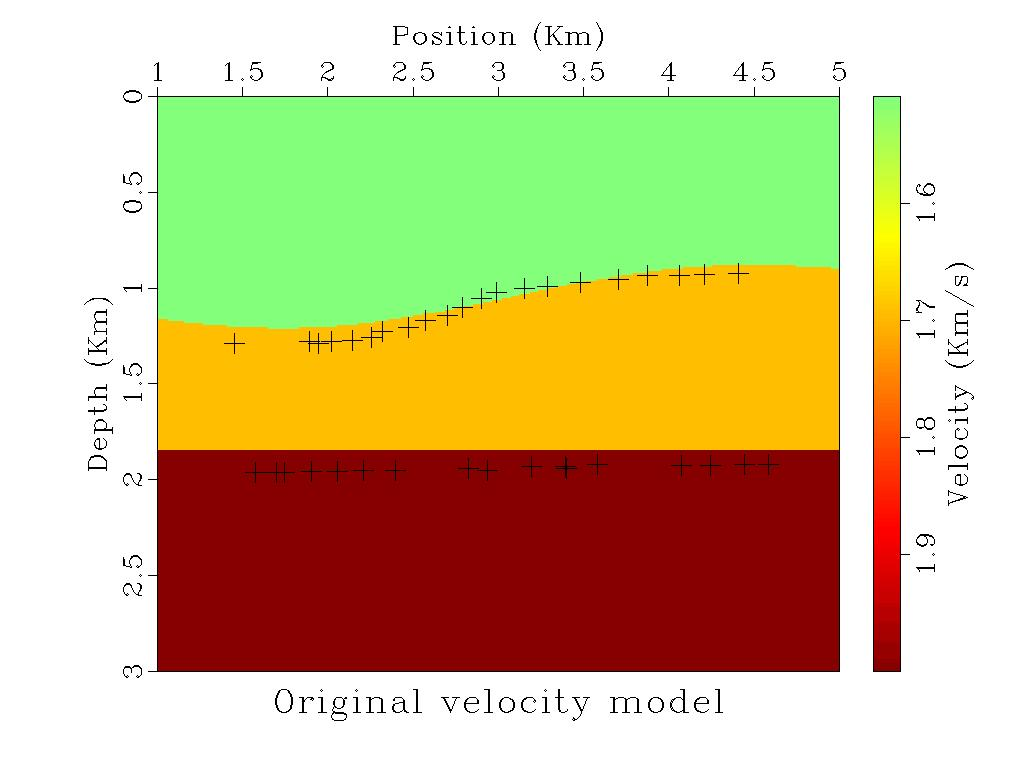
\includegraphics[scale=0.25]{images/gzvel.jpeg}
\vspace{-0.3cm}
\end{center}
\begin{center}
 Fonte: Do Autor.
\end{center}
\label{fig:11.3}
\end{figure}

\begin{figure}[H]
\caption{Resultado da localização das fontes PIN (cruzes em preto)
para o modelo de velocidades com perturbação sobre o modelo de velocidades original.}
\begin{center}
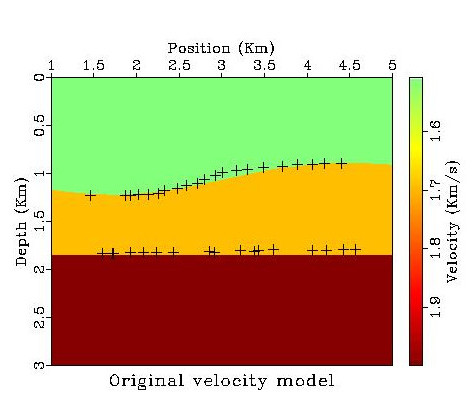
\includegraphics[scale=2.1]{images/endresult.jpeg}
\vspace{-0.3cm}
\end{center}
\begin{center}
 Fonte: Do Autor.
\end{center}
\label{fig:11.4}
\end{figure}

O resultado desta estratégia de otimização do modelo de velocidades é apresentado na Figura \ref{fig:11.2}.
Houve considerável melhora na localização das fontes pontuais PIN sobre os refletores (Ver
Figura \ref{fig:11.4}) em comparação com a etapa anterior do modelo de velocidades de
gradiente constante (Figura \ref{fig:11.3}).
Estes resultados indicam que a estratégia de inversão do modelo de velocidades utilizada é promissora, porém
que precisa ser elaborada uma melhor estratégia para a interpolação dos pontos sobre a malha do modelo de
velocidades e para suavizar o modelo (Figura \ref{fig:11.4}).

\chapter{CRONOGRAMA}
\label{cap9:cronograma}


\section{Etapas concluídas}

A seguir a descrição das etapas concluídas e o cronograma:

  \begin{enumerate}
   \item  Testes preliminares do algoritmos, Pesquisa e fundamentação teórica (09/2017 - 08/2019): Produção de testes 
   de implementação
   dos algoritmos utilizados e primeiras versões dos algoritmos originais do Autor.
   Pesquisa das principais referências teóricas e estabelecimento do tema central da tese.
   \item   Modelagem Kirchhoff (09/2019): Utilização do algoritmo de modelagem 
   do pacote Madagascar\footnote{Madagascar é um pacote
   de procesamento sísmico 'open source' disponível em \url{http://www.ahay.org/wiki/Main_Page}.}
   \textit{sfkirmod} para produzir os dados do modelo do refletor
   gaussiano.
    \item Obtenção dos parâmetros do SRC utilizando o VFSA (09/2019): Programa \textit{sfvfsacrenh} escrito  pelo Autor
    em linguagem C e adaptado para o pacote Madagascar
   baseado no algoritmo Very Fast Simulated Aneeling \cite{ingber}. O algoritmo ajusta a superfície de tempo de trânsito
   do SRC não hiperbólico (Equação \ref{eq:2.4}) aos dados modelados. Os parâmetros do SRC que produzem o melhor ajuste são
   os parâmetros otimizados.
    \item  Interpolação do cubo de dados com FPE (09/2019): Interpolação das seções de
    afastamento constante extraídas dos dados modelados
    (chamado ``cubo de dados'') a partir de Filtros Adaptativos de Predição de Erro
    com os programas \textit{sfapef} e \textit{sfmiss4} do pacote Madagascar.
    Esta interpolação permite a discretização
    suficiente dos traços no domínio do PMC para possibilitar a correta amostragem das famílias ERC.
    \item  Cálculo das trajetórias ERC (09/2019): Programa \textit{sfcretrajec} desenvolvido pelo Autor em linguagem C 
    e adaptado para o pacote Madagascar para
    o cálculo das trajetorias ERC baseado na Equação \ref{eq:2.1}.
     \item Obtenção das famílias ERC (09/2019): Programa \textit{sfgetcregather} desenvolvido pelo Autor em linguagem C 
     e adaptado para o pacote Madagascar para a
     determinação dos traços sísmicos do cubo de dados que estão sobre as trajetorias ERC previamente calculadas na etapa anterior.
     Estes traços formam as famílias ERC.
    \item  Cálculo das curvas de empilhamento ERC (10/2019): Programa \textit{sfgetcretimecurve} desenvolvido pelo Autor 
    em linguagem C e adaptado 
    para o pacote Madagascar para a determinação das curvas de tempo de trânsito ERC com auxílio das 
    Equações \ref{eq:2.3}-\ref{eq:2.4}.
     \item Paralelização do algoritmo com scons (12/2019): Utilização de técnicas de computação paralela para 
     melhorar o desempenho
     dos algoritmos desenvolvidos. O pacote Madagascar permite a Paralelização dos processos realizados a partir da execução
     com o comando \textit{scons -j\#} onde '\#' representa o número de núcleos utilizados.
    \item  Empilhamento e seção empilhada ERC (12/2019): Programa \textit{sfcrestack} 
    desenvolvido pelo Autor em linguagem C e adaptado 
    para o pacote Madagascar para a obtenção da seção  empilhada ERC.
  \end{enumerate}

    \begin{table}[H]
      \caption{Cronograma de trabalho das etapas já concluídas em cada mês do ano de 2019.}
      \centering
      
      \begin{tabular}{|p{6cm}|c|c|c|c|c|}%{|c|c|c|c|c|c|}

     \hline
      \textbf{Etapas concluídas} & 08/19 & 09/19 & 10/19 & 11/19 & 12/19 \\ \hline
      Pesquisa e fundamentação teórica & x & & &  & \\ \hline
      Modelagem Kirchhoff & & x & &  & \\ \hline
      Obtenção dos parâmetros do SRC utilizando o VFSA & & x & &  & \\ \hline
      Interpolação do cubo de dados com FPE & & x & &  & \\ \hline
      Cálculo das trajetórias ERC & & x & &  & \\ \hline
      Obtenção das famílias ERC & & x & &  & \\ \hline
      Cálculo das curvas de empilhamento ERC & & & x & & \\ \hline
      Paralelização do algoritmo com scons & & & & & x \\ \hline
      Empilhamento e seção empilhada ERC & & & &  & x \\
      \hline
      
      \end{tabular}
  \end{table}
  
A seguir as etapas concluídas após a qualificação de doutorado e até a entrega deste relatório:
  
  \begin{enumerate}
  \item Qualificação da tese (03/2020): Defesa e apresentação deste relatório de qualificação de tese.
  \item Desenvolvimento da estratégia de inversão do modelo de velocidades através da simulação
  de difrações \cite{diffractions}, esta estratégia foi abandonada, pois necessita do
  modelo de velocidades de sobretempo normal para simular as difrações (2020).
  \item Pesquisa teórica sobre a estratégia de inversão baseada na NIP tomografia \cite{niptomo}
  e stereotomografia \cite{stereo} e protótipos dos programas para o traçamento de raios (2020).
   \item Programas sfnipmodsetup e sfgetparameter desenvolvidos pelo Autor em linguagem C 
     e adaptados para o pacote Madagascar para a configuração inicial das fontes pontuais PIN
    e obtenção dos parâmetros $R_{NIP}$ e $\beta_0$ (03/2021).
   \item Desenvolvimento do programa sfzgradtomo desenvolvido pelo Autor em linguagem C 
    e adaptado para o pacote Madagascar para a inversão do modelo de velocidades de background
    (velocidade variando linearmente com a profundidade) (04/2021).
   \item Desenvolvimento do protótipo do programa sfstereoniptomo desenvolvido pelo Autor em linguagem C 
     e adaptado para o pacote Madagascar para a inversão do modelo de velocidades com variação
     lateral de velocidades (06/2021)
  \end{enumerate}


  \begin{table}[H]
      \caption{Cronograma de trabalho das etapas já concluídas em 2020 e 2021.}
      \centering
      
      \begin{tabular}{|p{6cm}|c|c|c|c|c|}%{|c|c|c|c|c|c|}

     \hline
      \textbf{Etapas concluídas} & 2020 & 03/21 & 04/21 & 05/21 & 06/21 \\ \hline
      Qualificação de doutorado & x & & &  & \\ \hline
      Inversão com simulação de difrações & x & & &  & \\ \hline
      Inversão baseada na NIP e stereo tomografia & x & & &  & \\ \hline
      Programas configuração inicial do modelo & & x & &  & \\ \hline
      Inversão modelo gradiente constante & & & x & x & \\ \hline
      Inversão variação lateral de velocidade (protótipo) & & & & & x \\
      \hline
      \end{tabular}
  \end{table}
  
\section{Etapas ainda não concluídas}

A seguir a descrição das atividades ainda não realizadas e o cronograma:

  \begin{enumerate}
    \item Inversão do modelo de velocidades com variação lateral (01/2022): Desenvolver o algoritmo de
    inversão do programa sfstereoniptomo completo.
    \item Testar a estratégia em outros modelos (02/2022): A estratégia de inversão será testada em 
    vários modelos de velocidades diferentes, em camadas com variações lateral de velocidade dentro da
    camada.
    \item  Escrita do texto da tese (08/2022): Escrever e revisar o texto da tese, apresentar os resultados da
    inversão do modelo de velocidades.
     \item Apresentação ao comitê de avaliação (08/2022): A data da apresentação para o Comitê de Avaliação de Tese é o dia 01 de Agosto de 2022.
    \item  Defesa de tese (08/2022): A data da apresentação para a Banca Avaliadora dependerá das sugestões do
    Comitê de Avaliação de Tese. A Previsão para defesa é entre os meses de Agosto de
    2022 e Setembro de 2022 (Já considerando a prorrogação do prazo de defesa).
  \end{enumerate}
  
   \begin{table}[H]
      \caption{Cronograma de trabalho até o prazo final da defesa de tese.}
      \centering
      
      \begin{tabular}{|p{6cm}|c|c|c|c|c|}

      \hline
      \textbf{Etapas ainda não concluídas} & 01/21 & 02/22 & 03/22 & 08/22 \\ \hline
      Inversão do modelo de velocidades & x & x & & \\ \hline
      Testes em vários modelos & & & x & \\ \hline
      Escrita do texto da tese & & & & x \\ \hline
      Apresentação ao comitê de avaliação & & & & x \\ \hline
      Defesa de tese & & & & x \\
      \hline
      
      \end{tabular}
  \end{table}
  
 % cronograma de atividades e entrega do trabalho
\chapter{CONCLUSÃO}
\label{cap10:conclusao}

As etapas já concluídas demonstram a que o método ERC pode ser utilizado para a obtenção da seção empilhada sem a necessidade
de informação a priori sobre o modelo de velocidades ou de uma etapa de análise de velocidades. Para melhor corroborar esta 
afirmação é necessário reproduzir o exeperimento aqui descrito com outros modelos iniciais, além do modelo do refletor gaussiano
aqui utilizado, e obter a seção de afastamento nulo.
Da forma como o algoritmo foi produzido, este deve ser capaz de produzir a seção empilhada mesmo para modelos de múltiplos refletores
com distribuições mais complexas de velocidade.

Nos resultados do empilhamento ERC no Capítulo \ref{cap7:empilhamento}, observamos que a forma do evento de reflexão na seção
de afastamento nulo foi preservada e as amplitudes foram realçadas. Porém, para testar como o algoritmo reage
a dados com ruído, é necessário reproduzir o experimento com diversos níveis de ruído aleatório adicionado aos dados modelados.

Outra observação é a de que o processo de empilhamento ERC adiciona ruído numérico aos traços da seção empilhada. Uma forma de
atenuar este ruído seria buscar uma maior precisão na determinação dos traços das famílias ERC: Aumentando a precisão das variáveis
nos programas (passando do tipo \textit{float} para \textit{double}, por exemplo), e realizando a interpolação e regularização
mais de uma vez nos dados modelados até que a discretização seja satisfatória.

Enfim, os resultados deste trabalho serão publicados em dois artigos científicos: O primeiro baseado 
nos resultados obtidos e e os que 
serão obtidos da repetição deste experimento para modelos mais complexos, este irá focar no método ERC e na obtenção da seção
empilhada ERC a partir da aplicação da condição SDC à aproximação não hiperbólica do tempo de trânsito SRC (Equação \ref{eq:2.4}).
O segundo artigo irá tratar da inversão do modelo de velocidades a partir da metodologia de inversão aqui proposta
no Capítulos 9 a 11.

As etapas já concluídas demonstram que a estratégia de inversão do modelo de velocidades é promissora,
pois permite localizar corretamente as fontes pontuais PIN sobre os refletores em profundidade
e obter um modelo de velocidades suavizado que pode ser utilizado como primeiro passo
para a construção do modelo de velocidades em profundidade. Todavia,
esta estratégia necessita de uma melhor forma de representar o modelo de velocidades com variação lateral
de velocidades e metodologia de interpolação.

O critério de convergência utilizado também precisa ser alterado para poder tratar modelos mais complexos.
Neste relatório utilizamos as diferenças entre o tempo de trânsito obtido no traçamento de raios e a fórmula
do ERC. Porém, a fórmula do ERC depende dos parâmetros $R_{NIP}$ e $\beta_0$ obtidos durante o empilhamento ERC.
A incerteza na determinação destes parâmetros resulta em incerteza na determinação da localização das fontes
pontuais PIN durante a inversão e na determinação dos tempos de trânsito com a fórmula ERC. Por isso, seria
melhor utilizar o semblance calculado nas famílias ERC nos dados pré-empilhados, ajustando as curvas de tempo
de trânsito obtidas no traçamento de raios aos dados.

Por fim, para cumprir os objetivos estabelecidos no cronograma deste relatório solicito a prorrogação do prazo de defesa da minha tese de doutorado por mais um ano além do prazo normal de defesa. Os motivos do atraso no 
desenvolvimento da tese foram explicitados na justificativa e oque foi desenvolvido desde a interrupção
das atividades laboratoriais por causa da pandemia de Covid-19 também foi devidamente apresentado neste relatório.
 % conclusão discutindo os resultados obtidos e esperados

\bookmarksetup{startatroot}

\bibliography{mybib}

%% Inicia os apêndices
%% ---
\begin{apendicesenv}

%% Imprime uma página indicando o início dos apêndices
\partapendices
%\newpage\null\thispagestyle{empty}
% \begin{center}
% \vspace{10cm}
% {\large\textbf{APÊNDICES}}
% \end{center}
% \newpage

\input{apendice_tempo_transito_cre}
% \input{apendiceB}
% \input{apendiceC}
% \input{apendiceD}
% \input{MT}
%
\end{apendicesenv}

%% Inicia os anexos
%\begin{anexosenv}
%\partanexos
%\include{AnexoA}

%\end{anexosenv}

\cleardoublepage
\phantomsection 
\printindex

\end{document}
